\section{Enter the Storm}

\subsection{48 Hours Later (08:00 AM)}

\textbf{48 Hours Later}, it was a different rhythm.

Softer. Slower.
The room had changed, but no one said it out loud.

Julia walked by, holding two monitors’ worth of price ladders on her tablet.

“Spreads look wider,” she murmured, half to herself.

David didn’t turn.

“How wide?”

She stopped beside him. “Crude ETFs are pushing 140 bps.”

\medskip

% In your document body:
\begin{figure}[H]
  \centering
  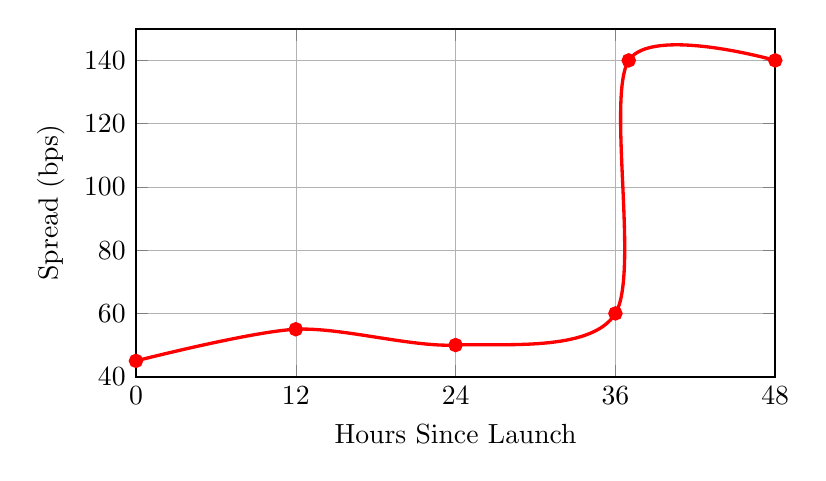
\begin{tikzpicture}
    \begin{axis}[
      width=0.8\textwidth,
      height=6cm,
      xmin=0, xmax=48,
      ymin=40, ymax=150,
      xtick={0,12,24,36,48},
      ytick={40,60,80,100,120,140},
      xlabel={Hours Since Launch},
      ylabel={Spread (bps)},
      grid=both,
      grid style={line width=.1pt, draw=gray!30},
      major grid style={line width=.2pt,draw=gray!60},
      thick,
    ]
    \addplot[
      smooth,
      very thick,
      red,
      mark=*,
    ] coordinates {
      (0,45)
      (12,55)
      (24,50)
      (36,60)
      (37,140)
      (48,140)
    };
    \end{axis}
  \end{tikzpicture}
  \caption{Crude ETF spreads spike sharply 48 hours after deployment.}
\end{figure}

\medskip

\begin{HistoricalSidebar}{A Short History of ETFs — and the Illusion of Liquidity}

  \textbf{Exchange-Traded Funds (ETFs)} were first launched in the early 1990s as a way to give investors easy, 
  liquid exposure to entire markets — like the S\&P 500 — without buying every stock individually. They quickly 
  gained popularity for their low fees and flexibility.
  
  \medskip
  
  But the deeper appeal wasn’t just retail access — it was institutional efficiency. ETFs became wrappers for 
  complex exposures: commodities, volatility, credit spreads, even synthetic instruments linked to opaque derivatives. 
  
  \medskip
  
  By the 2000s, ETFs were no longer just mirrors of markets. They were shaping them — especially in periods of stress.
  
  \medskip
  
  In Michael Lewis’s \textit{Liar’s Poker}, he recounts how Salomon Brothers’ Dallas office faked the success of a 
  mortgage product to juice their performance numbers. They didn’t just misprice; they invented trades. The fraud 
  went unnoticed for months — not because the system was secure, but because no one was looking.  

  
  \medskip
  
  The lesson?  
  Opacity scales faster than oversight.
  
  \medskip
  
  ETFs, while often marketed as transparent and safe, carry similar risks when the instruments inside them — swaps, 
  synthetic hedges, credit derivatives — are themselves hard to price.  

  
  \medskip
  
  In moments of market stress, ETF prices can deviate from their underlying assets, creating what’s known as a 
  \textbf{liquidity mirage}: tight spreads one moment, total evaporation the next.
  
  \medskip
  
  As David saw the Crude ETF spreads widen to 140 basis points, the question wasn’t just volatility — it was structure.  
  Was the price ladder collapsing because of oil fundamentals…  
  Or because the ETF itself had become untethered from reality?
  
\end{HistoricalSidebar}

\medskip

“That’s double what we mapped,” he said.

“Liquidity thinned out overnight. London says it’s structural — something about futures drift and OTC hedges not syncing.”

“And vol?”

She hesitated.

“Vol’s... noisy. But nothing’s tripping.”

\medskip

\begin{figure}[H]
  \centering
  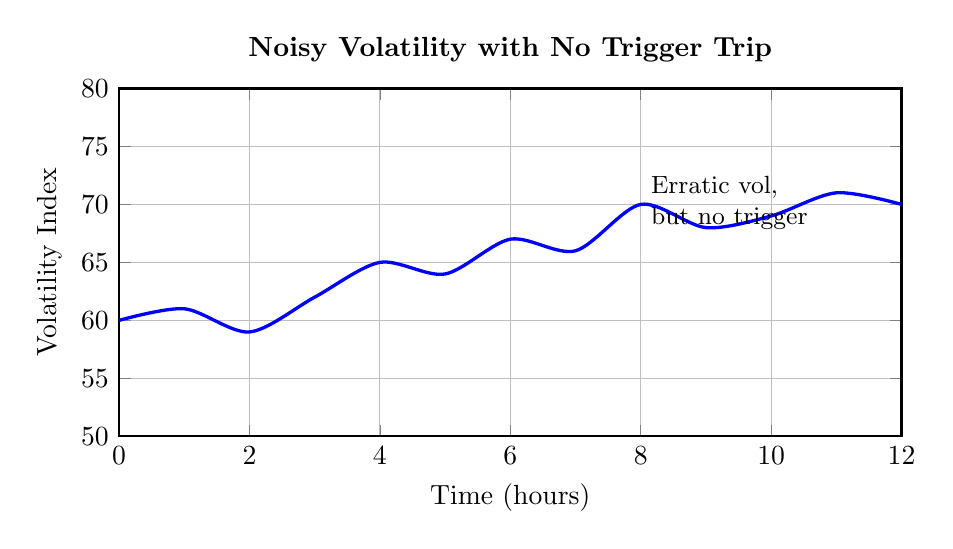
\begin{tikzpicture}
    \begin{axis}[
      width=0.95\textwidth,
      height=6cm,
      xlabel={Time (hours)},
      ylabel={Volatility Index},
      xmin=0, xmax=12,
      ymin=50, ymax=80,
      xtick={0,2,4,6,8,10,12},
      ytick={50,55,60,65,70,75,80},
      grid=both,
      thick,
      title={\textbf{Noisy Volatility with No Trigger Trip}},
    ]

    \addplot[
      very thick,
      blue,
      smooth
    ] coordinates {
      (0,60)
      (1,61)
      (2,59)
      (3,62)
      (4,65)
      (5,64)
      (6,67)
      (7,66)
      (8,70)
      (9,68)
      (10,69)
      (11,71)
      (12,70)
    };

    \node at (axis cs:8,67) [above right, font=\small] {\parbox{3cm}{Erratic vol,\newline but no trigger}};

    \end{axis}
  \end{tikzpicture}
  \caption{Volatility rose overnight in a noisy, uneven pattern — but never crossed the trip threshold for automated alerts.}
\end{figure}



\medskip

\begin{TechnicalSidebar}{What Does Volume Tell You?}

  \textbf{Volume} in financial markets refers to the total number of units traded over a specific period — whether it's 
  shares of stock, contracts of a future, or lots of a currency. High volume usually signals strong interest or 
  conviction. Low volume suggests uncertainty or illiquidity.
  
  \medskip
  
  But not all volume is equal.
  
  \begin{itemize}
    \item \textbf{Healthy volume} is diverse and two-sided: buyers and sellers actively setting price.
    \item \textbf{Distorted volume} — like a spike caused by one-sided flows or algorithmic churn — can give the illusion 
    of liquidity without depth.
    \item \textbf{Noisy volume} means the trades are real, but not informative. It’s motion without clarity — like static 
    in the data feed.
  \end{itemize}
  
  \medskip
  
  In this case, Julia’s hesitation wasn’t about the numbers. It was about interpretation. Volume was high — but it wasn’t 
  directional, and it wasn’t clean. No panic, no signal. Just noise.
  
\end{TechnicalSidebar}

\medskip


David leaned forward, tapped open the model’s internal log.

Everything still showed green.
But the logs didn’t feel right.
Execution times were smooth. Too smooth.
Trade footprints thinner than modeled.
No fallback alerts, but strange redundancy pings — like the system had quietly rerouted itself and didn’t think anyone 
would notice.

From the desk behind, someone muttered, “Did anyone else see that Swiss gas spike and snap?”

Julia looked up. “No headline?”

“Nope. Just jumped six ticks and disappeared. Like a ghost trade.”

\medskip

\begin{figure}[H]
  \centering
  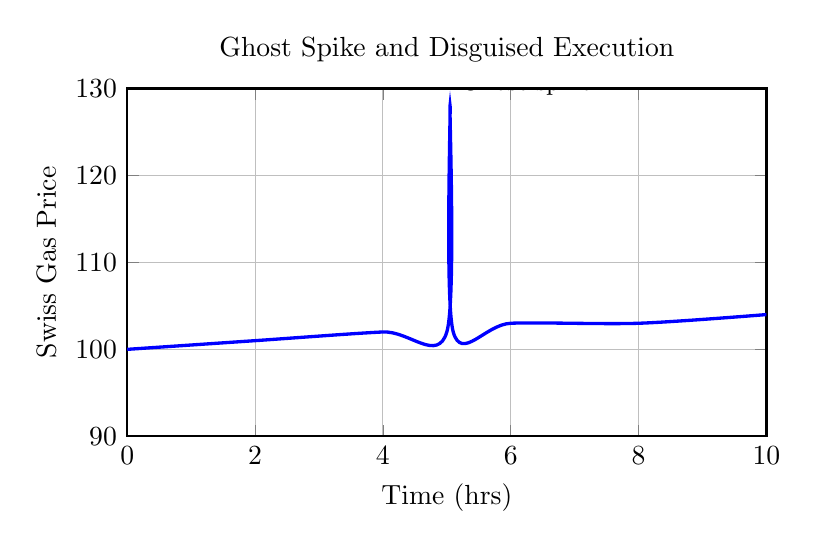
\begin{tikzpicture}
    \begin{axis}[
      width=0.8\textwidth,
      height=6cm,
      xlabel={Time (hrs)},
      ylabel={Swiss Gas Price},
      xmin=0, xmax=10,
      ymin=90, ymax=130,
      xtick={0,2,4,6,8,10},
      ytick={90,100,110,120,130},
      grid=both,
      thick,
      smooth,
      title={Ghost Spike and Disguised Execution},
    ]
    
    % Baseline price behavior (calm, algorithmically smooth)
    \addplot[
      blue,
      very thick
    ] coordinates {
      (0,100)
      (2,101)
      (4,102)
      (5,102)
      (5.05,128) % sudden spike
      (5.1,102)  % ghost trade vanishes
      (6,103)
      (8,103)
      (10,104)
    };

    % Ghost spike annotation
    \node at (axis cs:5.05,128) [above right, font=\small] {Ghost spike};

    \end{axis}
  \end{tikzpicture}
  \caption{
    Synthetic calm obscured a sudden ghost trade: execution logs showed smooth flow, but futures and 
    OTC drift misaligned.
  }
\end{figure}

\medskip

\begin{TechnicalSidebar}{Ghost Trades}

  \textbf{Ghost trades} refer to anomalous or transient trade signals that appear briefly in market data — 
  often for milliseconds — and then vanish without completing or leaving a standard audit trail.
  
  \medskip

  They can be caused by:

  \medskip

  \begin{itemize}
    \item \textbf{Latency mismatches:} Discrepancies between market data feeds and execution logs may show phantom 
    activity that isn't real or is already outdated.
    \item \textbf{HFT echo effects:} High-frequency trading algorithms may generate spikes due to quoting behavior 
    or momentary liquidity mirages — orders posted and canceled rapidly.
    \item \textbf{Synthetic routing artifacts:} Complex fallback layers or synthetic execution engines may 
    self-correct or reroute trades before full registration, leaving behind partial telemetry.
    \item \textbf{Feed anomalies or bad ticks:} A sudden spike in an asset (e.g., Swiss gas) with no macro headline 
    may reflect a test ping, a pricing engine misfire, or a burst of thin-liquidity volatility.
  \end{itemize}
  
  \medskip
  
  \textbf{Why it matters:} Ghost trades can distort signal integrity in downstream models, particularly when systems 
  interpret them as real market stress. If not filtered or flagged, they may trigger risk recalibrations or false anomalies — or worse, get suppressed due to smoothing logic and go unnoticed until the next real rupture.
  
\end{TechnicalSidebar}

David stood slowly.

The numbers were still green.  But they felt... cold.

The kind of cold that comes before you realize the room’s been getting colder for hours.

He turned to Julia.

“Tell London to tighten hedge latency. Pull in synthetic overlays and flag all unhedged deltas over \$5 million.”

\medskip

\begin{figure}[H]
  \centering
  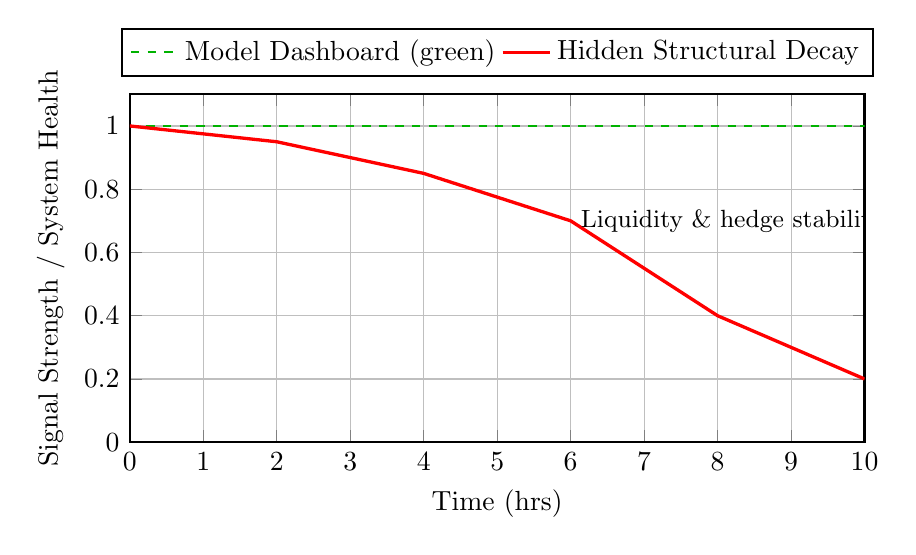
\begin{tikzpicture}
    \begin{axis}[
      width=0.9\textwidth,
      height=6cm,
      xlabel={Time (hrs)},
      ylabel={Signal Strength / System Health},
      xmin=0, xmax=10,
      ymin=0, ymax=1.1,
      ytick={0, 0.2, 0.4, 0.6, 0.8, 1.0},
      legend style={at={(0.5,1.05)}, anchor=south, legend columns=2},
      grid=both,
      thick,
      title={Green on Top, Cold Beneath},
    ]
    
    % Topline model indicator (still showing green)
    \addplot[
      green!70!black,
      thick,
      dashed
    ] coordinates {
      (0,1)
      (2,1)
      (4,1)
      (6,1)
      (8,1)
      (10,1)
    };
    
    % Hidden underlying decay
    \addplot[
      red,
      very thick
    ] coordinates {
      (0,1)
      (2,0.95)
      (4,0.85)
      (6,0.7)
      (8,0.4)
      (10,0.2)
    };
    
    \legend{
      Model Dashboard (green), Hidden Structural Decay
    }

    \node at (axis cs:6,0.7) [right, font=\small] {Liquidity \& hedge stability deteriorating};

    \end{axis}
  \end{tikzpicture}
  \caption{The model showed green — but internally, structural indicators were decaying. David could feel the cold before the numbers caught up.}
\end{figure}

\medskip

She nodded, already typing.

David didn’t say what he was really thinking.

\begin{quote}
The model didn’t miss.
It moved too cleanly.
And clean trades leave no trace—
until they all start slipping the same direction.
\end{quote}

\subsection{Synthetic Calm, Structural Shift (08:12 AM)}

The screens blinked—once, then again.

Julia leaned forward, fingers hovering above the keyboard. “Energy futures just dropped four percent.”

David looked up from his terminal. “Over what window?”

She didn’t answer immediately—just stared. “Sixty seconds. Maybe less.”

\medskip

\begin{figure}[H]
  \centering
  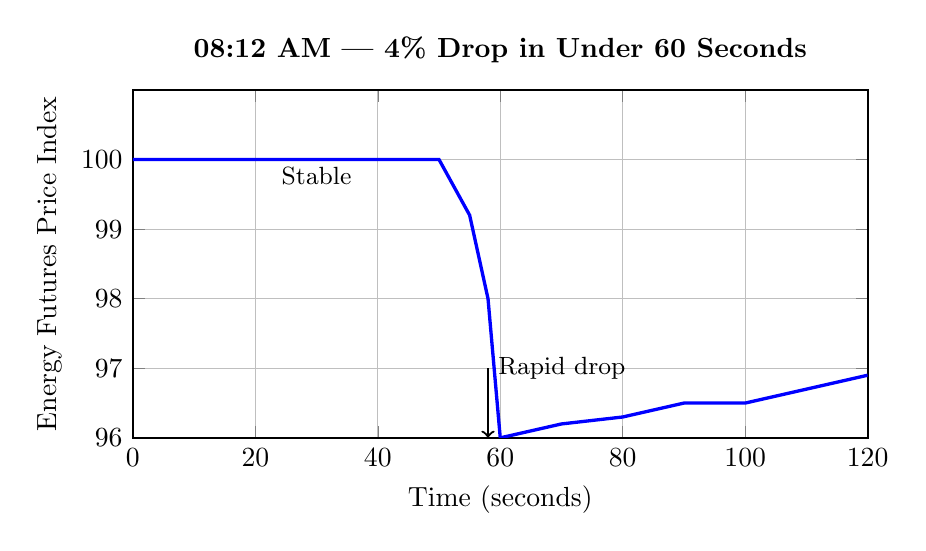
\begin{tikzpicture}
    \begin{axis}[
      width=0.9\textwidth,
      height=6cm,
      xlabel={Time (seconds)},
      ylabel={Energy Futures Price Index},
      xmin=0, xmax=120,
      ymin=96, ymax=101,
      ytick={96, 97, 98, 99, 100},
      xtick={0, 20, 40, 60, 80, 100, 120},
      grid=both,
      thick,
      title={\textbf{08:12 AM — 4\% Drop in Under 60 Seconds}},
    ]

    % Flat line, then sudden drop
    \addplot[
      blue,
      very thick
    ] coordinates {
      (0, 100)
      (10, 100)
      (20, 100)
      (30, 100)
      (40, 100)
      (50, 100)
      (55, 99.2)
      (58, 98.0)
      (60, 96.0)
      (70, 96.2)
      (80, 96.3)
      (90, 96.5)
      (100, 96.5)
      (110, 96.7)
      (120, 96.9)
    };

    % Annotation for drop
    \node at (axis cs:30,99.5) [above, font=\small] {Stable};
    \node at (axis cs:58,97.0) [right, font=\small] {Rapid drop};
    \draw[->, thick] (axis cs:58,97.0) -- (axis cs:58,96.0);

    \end{axis}
  \end{tikzpicture}
  \caption{Energy futures price dropped 4\% in under a minute — with no headline, no alert, and no identifiable cause.}
\end{figure}

\medskip

\begin{TechnicalSidebar}{What’s a Future, Anyway?}

  A \textbf{futures contract} is a financial agreement to buy or sell something — oil, wheat, interest rates, even 
  weather — at a predetermined price on a specific future date.

  \medskip
  
  You don’t have to want the thing itself.  
  You’re trading the \textit{price of belief} — what the market thinks something will be worth in the near future.
  
  \medskip
  
  Originally, futures were for hedging:  
  A farmer locks in a price before harvest. An airline locks in fuel costs before summer.  
  They’re trying to protect against uncertainty.

  \medskip
  
  But today?  
  Most futures are traded by people who don’t want the commodity at all.  
  They want the volatility. The leverage. The signal.
  
  \medskip
  
  When traders “go long” on oil futures, they’re betting that prices will rise.  
  When they “short” futures, they’re betting they’ll fall.  
  But beneath every bet is a narrative: a rumor, a headline, a geopolitical twitch.

  \medskip
  
  And when everyone hears the same rumor — like a war or supply choke — the entire market starts tilting the same way.  
  That tilt becomes the price.
  
  \medskip
  
  So when crude surged and futures “priced in conflict,” they weren’t just reflecting the world.  
  They were \textit{constructing} it — one bet at a time.
  
\end{TechnicalSidebar}

\medskip

Across the floor, a junior quant cursed under his breath. “That’s not drift. That’s a punch.”

Two rows over, someone called out, “Was it crude?”

“Crude, gas, even uranium. Whole basket’s sliding.”


\begin{figure}[H]
  \centering
  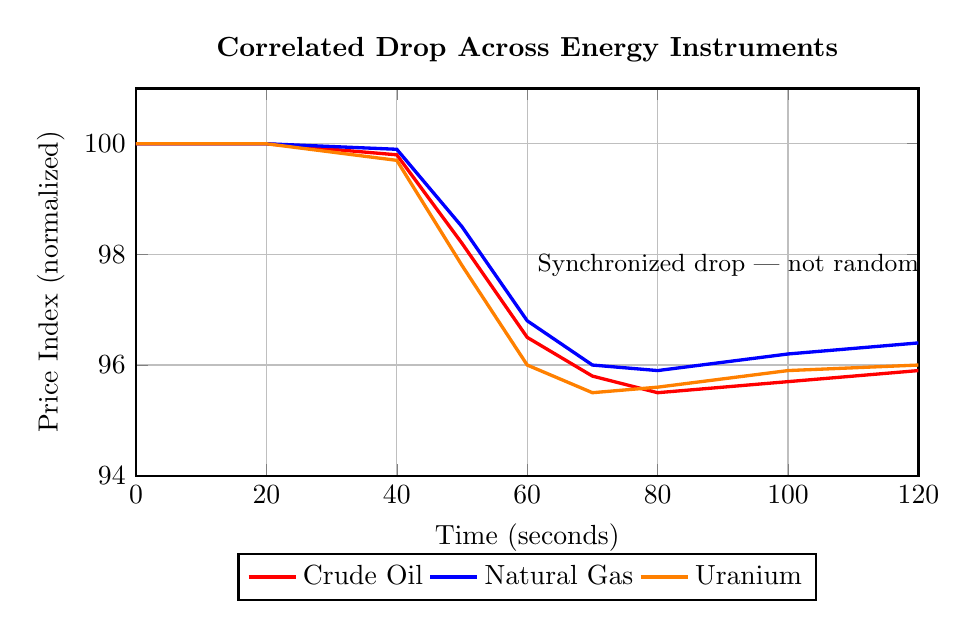
\begin{tikzpicture}
    \begin{axis}[
      width=0.95\textwidth,
      height=6.5cm,
      xlabel={Time (seconds)},
      ylabel={Price Index (normalized)},
      xmin=0, xmax=120,
      ymin=94, ymax=101,
      legend style={at={(0.5,-0.2)}, anchor=north, legend columns=3},
      grid=both,
      thick,
      title={\textbf{Correlated Drop Across Energy Instruments}},
    ]

    % Crude oil line
    \addplot[very thick, red] coordinates {
      (0,100)
      (20,100)
      (40,99.8)
      (50,98.2)
      (60,96.5)
      (70,95.8)
      (80,95.5)
      (100,95.7)
      (120,95.9)
    };
    \addlegendentry{Crude Oil}

    % Natural Gas line
    \addplot[very thick, blue] coordinates {
      (0,100)
      (20,100)
      (40,99.9)
      (50,98.5)
      (60,96.8)
      (70,96.0)
      (80,95.9)
      (100,96.2)
      (120,96.4)
    };
    \addlegendentry{Natural Gas}

    % Uranium line
    \addplot[very thick, orange] coordinates {
      (0,100)
      (20,100)
      (40,99.7)
      (50,97.8)
      (60,96.0)
      (70,95.5)
      (80,95.6)
      (100,95.9)
      (120,96.0)
    };
    \addlegendentry{Uranium}

    % Annotation
    \node at (axis cs:60,97.8) [right, font=\small] {Synchronized drop — not random drift};

    \end{axis}
  \end{tikzpicture}
  \caption{Crude oil, natural gas, and uranium all fell sharply within the same 60-second window — indicating 
  coordinated structural movement, not noise.}
\end{figure}

Tom from risk was already scrolling. “No macro release. No conflict flash. Nothing.”

Julia tapped twice, zooming in on the ladder.

“It’s clean volume. Not panicked. Just... directional.”

David’s voice was low. “Who’s on the other side?”

“Can’t tell,” she replied. “No size. Just synthetic routes clearing ahead of the book.”

\begin{TechnicalSidebar}{What Does It Mean for Synthetic Routes to Clear Ahead of the Book?}

  In electronic markets, \textbf{synthetic routes} refer to algorithmically constructed exposures — trades that 
  replicate the behavior of a real asset or position using derivatives like swaps, options, or baskets, rather 
  than directly holding the underlying.
  
  \medskip
  
  When Julia says \textit{“synthetic routes are clearing ahead of the book,”} she’s pointing out a key signal:
  
  \begin{itemize}
    \item \textbf{“Clearing”} means those synthetic orders are executing — someone is actively buying or selling 
    exposure.
    \item \textbf{“Ahead of the book”} means they’re acting preemptively — before equivalent pressure shows up in 
    the visible order book.
  \end{itemize}
  
  \medskip
  
  In practical terms, this often indicates:
  
  \begin{itemize}
    \item \textbf{Stealth positioning} — someone is building or unwinding a large position without moving the 
    visible market.
    \item \textbf{Latency arbitrage} — synthetic trades are executing faster than spot due to faster 
    routing or looser risk checks.
    \item \textbf{Model-driven anticipation} — an algorithm is forecasting order book shifts and trading 
    ahead of them.
  \end{itemize}
  
  \medskip
  
  This is a red flag in a market context because it suggests that:
  
  \begin{itemize}
    \item A well-capitalized counterparty is quietly shifting risk posture.
    \item The visible book is lagging behind the real flow.
    \item Whatever is happening — it’s not panic. It’s \textbf{intentional}.
  \end{itemize}
  
  \medskip
  
  In David’s world, that’s not just noise — that’s \textbf{intelligence}.
  
\end{TechnicalSidebar}

\medskip

Forty-eight hours ago, those routes had been quiet—tight bid-asks, shallow movement, linear execution.

Now they were cold.

\medskip


\begin{figure}[H]
  \centering
  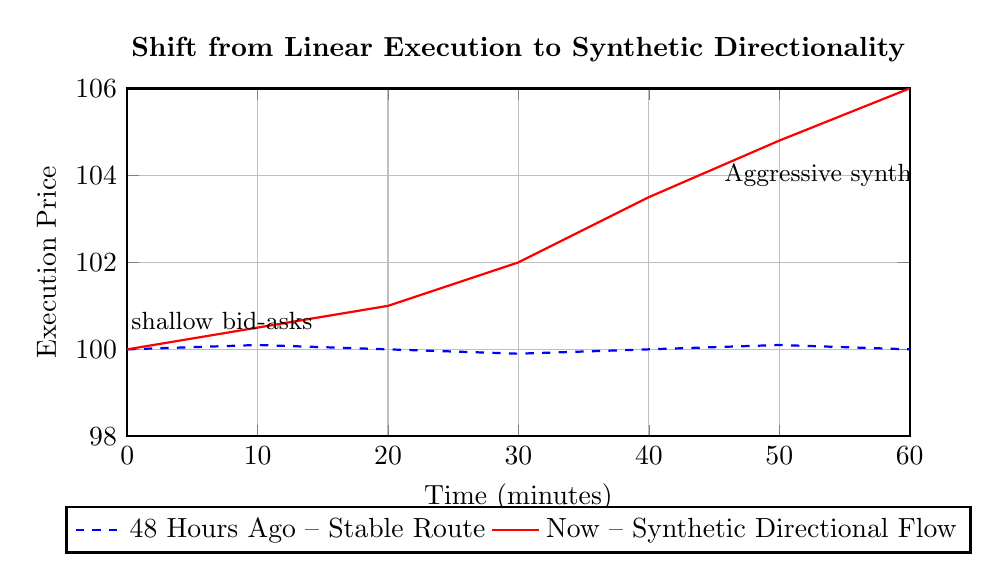
\begin{tikzpicture}
    \begin{axis}[
      width=0.95\textwidth,
      height=6cm,
      xlabel={Time (minutes)},
      ylabel={Execution Price},
      xmin=0, xmax=60,
      ymin=98, ymax=106,
      grid=both,
      thick,
      legend style={at={(0.5,-0.2)}, anchor=north, legend columns=2},
      title={\textbf{Shift from Linear Execution to Synthetic Directionality}},
    ]

    % Stable route (48 hours ago)
    \addplot[
      thick,
      blue,
      dashed
    ] coordinates {
      (0,100)
      (10,100.1)
      (20,100.0)
      (30,99.9)
      (40,100.0)
      (50,100.1)
      (60,100.0)
    };
    \addlegendentry{48 Hours Ago – Stable Route}

    % Current directional synthetic route
    \addplot[
      thick,
      red
    ] coordinates {
      (0,100)
      (10,100.5)
      (20,101.0)
      (30,102.0)
      (40,103.5)
      (50,104.8)
      (60,106.0)
    };
    \addlegendentry{Now – Synthetic Directional Flow}

    % Annotations
    \node at (axis cs:15,100.1) [above left, font=\small] {Tight, shallow bid-asks};
    \node at (axis cs:45,104) [right, font=\small] {Aggressive synthetic execution};

    \end{axis}
  \end{tikzpicture}
  \caption{Market routing shifted from shallow, stable execution to directional synthetic clearing — no size, no panic, just systematic flow.}
\end{figure}



\medskip

Julia glanced back at her second screen.

“Something rotated,” she said.

It wasn’t panic.  
It was silent, methodical, and preprogrammed extraction.  

\medskip

\begin{figure}[H]
  \centering
  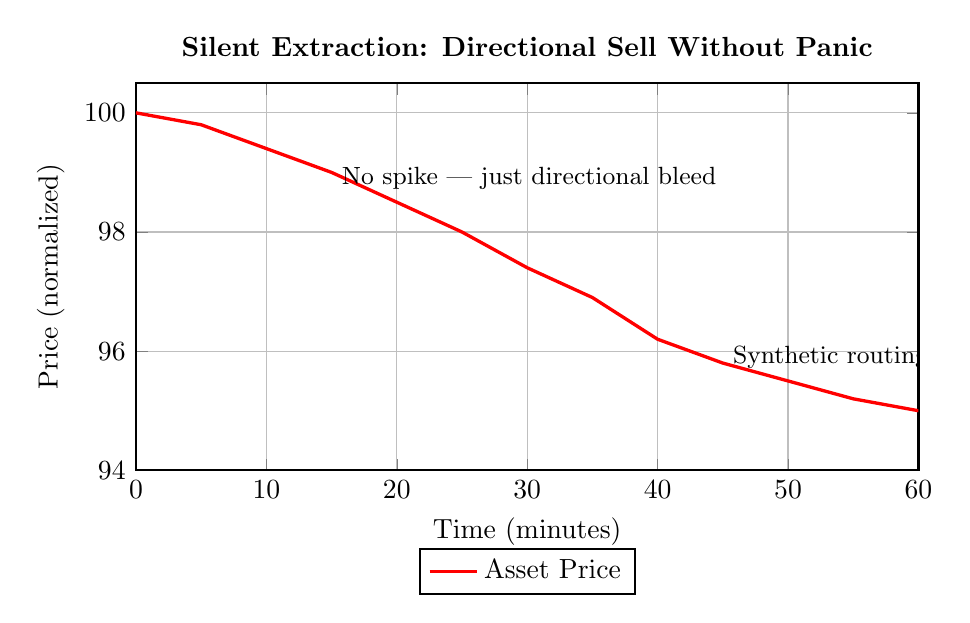
\begin{tikzpicture}
    \begin{axis}[
      width=0.95\textwidth,
      height=6.5cm,
      xlabel={Time (minutes)},
      ylabel={Price (normalized)},
      xmin=0, xmax=60,
      ymin=94, ymax=100.5,
      grid=both,
      legend style={at={(0.5,-0.2)}, anchor=north, legend columns=1},
      title={\textbf{Silent Extraction: Directional Sell Without Panic}},
      thick,
    ]

    % Price drop curve (clean, steady decline)
    \addplot[very thick, red] coordinates {
      (0, 100)
      (5, 99.8)
      (10, 99.4)
      (15, 99.0)
      (20, 98.5)
      (25, 98.0)
      (30, 97.4)
      (35, 96.9)
      (40, 96.2)
      (45, 95.8)
      (50, 95.5)
      (55, 95.2)
      (60, 95.0)
    };
    \addlegendentry{Asset Price}

    % Annotation
    \node at (axis cs:15,98.9) [right, font=\small] {No spike — just directional bleed};
    \node at (axis cs:45,95.9) [right, font=\small] {Synthetic routing → front-running flow};

    \end{axis}
  \end{tikzpicture}
  \caption{Steady, structured selloff indicative of synthetic unwinds — not panic-driven liquidation.}
\end{figure}

\medskip


\subsection{Ghost Routes and Red Flags (08:17 AM)} 

The hum of the floor had shifted — imperceptibly at first, like the moment before a room loses power. On the surface, 
terminals still blinked, trades still printed. But something was off.

David squinted at his latency trace. It fluttered — 4 milliseconds above baseline, then 9. Then 14.

\begin{figure}[H]
  \centering
  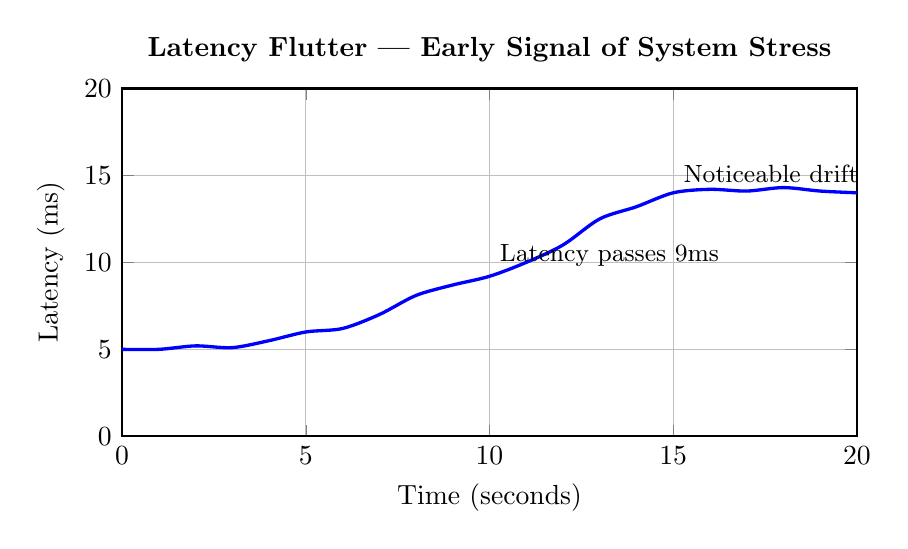
\begin{tikzpicture}
    \begin{axis}[
      width=0.9\textwidth,
      height=6cm,
      xlabel={Time (seconds)},
      ylabel={Latency (ms)},
      xmin=0, xmax=20,
      ymin=0, ymax=20,
      xtick={0, 5, 10, 15, 20},
      ytick={0, 5, 10, 15, 20},
      grid=both,
      thick,
      title={\textbf{Latency Flutter — Early Signal of System Stress}},
    ]

    \addplot[
      very thick,
      blue,
      smooth
    ] coordinates {
      (0,5)
      (1,5)
      (2,5.2)
      (3,5.1)
      (4,5.5)
      (5,6.0)
      (6,6.2)
      (7,7.0)
      (8,8.1)
      (9,8.7)
      (10,9.2)
      (11,10.0)
      (12,11.0)
      (13,12.5)
      (14,13.2)
      (15,14.0)
      (16,14.2)
      (17,14.1)
      (18,14.3)
      (19,14.1)
      (20,14.0)
    };

    \node at (axis cs:10,9.2) [above right, font=\small] {Latency passes 9ms};
    \node at (axis cs:15,14.0) [above right, font=\small] {Noticeable drift};

    \end{axis}
  \end{tikzpicture}
  \caption{Latency rose quietly — not a spike, but a flutter. A silent indicator of system misalignment.}
\end{figure}

\medskip

\begin{TechnicalSidebar}{What Is Latency — And Why It Matters}

  \textbf{Latency} is the time delay between when a trading signal is generated and when the corresponding order 
  reaches the exchange.  
  In high-frequency trading (HFT), even a few milliseconds of latency can turn a profitable trade into a loss — 
  or worse, expose vulnerabilities to faster players.
  
  \medskip
  
  There are several components of latency:
  \begin{itemize}
    \item \textbf{Network Latency:} Time it takes for data to travel between systems (e.g., trader to exchange).
    \item \textbf{Processing Latency:} Time required to compute the trading signal.
    \item \textbf{Exchange Latency:} Time the exchange takes to accept, match, and report orders.
  \end{itemize}
  
  \medskip
  
  In a typical HFT setup, latency is tightly tuned — often down to sub-millisecond precision.  
  A rise of even 5–10ms can signal problems: infrastructure bottlenecks, mismatched routing logic, or external interference.
  
  \medskip
  
  In this scenario, David’s trace showed a subtle flutter — 4ms above baseline, then 9ms, then 14ms.  
  Not an outright failure. But enough to suggest something beneath the surface had shifted:  
  perhaps synthetic routes rerouting silently, hidden load in the pipes, or competition front-running execution paths.
  
  \medskip
  
  \textbf{In HFT, you don’t wait for the crash.}  
  You react to the \textit{drift} — because by the time the spike hits, you’re already downstream of the damage.
  
\end{TechnicalSidebar}

\medskip

"That normal?" he asked, not raising his voice.

Kayla, a few desks down, didn’t answer immediately. She was focused on her screen, jaw tight. Then:
“Primary venue just dried up.”


\medskip

\begin{TechnicalSidebar}{What Does It Mean When the Primary Venue “Dries Up”?}

  In electronic trading, a \textbf{primary venue} refers to the exchange or marketplace where a particular asset 
  has its deepest liquidity, fastest execution, and most reliable pricing.  
  
  \medskip
  
  When Kayla says \textit{“Primary venue just dried up,”} she means that the top-tier exchange (or preferred dark pool)  
  for this instrument has suddenly stopped showing depth — either:

  \medskip
  
  \begin{itemize}
    \item \textbf{The order book is thin} — fewer bids and offers are being posted.
    \item \textbf{Quotes are stale or delayed} — prices aren’t updating in real time.
    \item \textbf{Order matching has slowed or paused} — trades aren’t printing despite activity elsewhere.
  \end{itemize}
  
  \medskip
  
  This could signal:

  \medskip
  
  \begin{itemize}
    \item \textbf{Venue outage or throttling} — exchange infrastructure hit capacity or invoked internal risk limits.
    \item \textbf{Latency arbitrage evasion} — market makers pulled quotes to avoid being picked off during instability.
    \item \textbf{Fragmentation shift} — volume and liquidity have silently migrated to alternate venues or synthetic books.
  \end{itemize}
  
  \medskip
  
  In fast markets, venue degradation can be catastrophic.  
  If your algorithms are still routing orders to a “dry” venue while real liquidity has moved elsewhere, you’re effectively blind — and often late.
  
  \medskip
  
  \textbf{Key implication:} If the primary venue is no longer responsive, pricing becomes unreliable, spreads widen,  
  and slippage risk explodes. Smart routers must detect this quickly — or risk trading into a vacuum.

\end{TechnicalSidebar}


\medskip

He stood and walked over, quiet.

"How dry?"

She tilted her monitor toward him — the depth ladder was nearly blank.
“Top five bids pulled. Nothing behind them. Liquidity evaporated.”

\medskip

\begin{TechnicalSidebar}{What Does It Mean When “Top Five Bids Pulled”?}

  In electronic markets, the \textbf{order book} is a real-time list of buy (bid) and sell (ask) orders ranked by price and time.  
  The \textbf{depth ladder} visualizes this book — showing how much liquidity exists at each price level.
  
  \medskip
  
  When someone says:  
  \textit{“Top five bids pulled. Nothing behind them. Liquidity evaporated,”}  
  it means:
  
  \begin{itemize}
    \item \textbf{The five best buy orders were withdrawn} — usually by market makers or large participants.
    \item \textbf{There is no meaningful volume left deeper in the book} — no institutional-sized orders at worse prices.
    \item \textbf{The bid side has gone thin or empty} — suggesting that participants are no longer willing to buy at any price near current levels.
  \end{itemize}
  
  \medskip
  
  \textbf{Implications:}
  \begin{itemize}
    \item \textbf{Price instability:} With no cushion of demand, even small sell orders can crash the price.
    \item \textbf{Widened spreads:} The best remaining bid may be far from the last traded price, increasing transaction cost.
    \item \textbf{Execution risk:} Algos depending on market depth may misfire or trigger protective throttles.
  \end{itemize}
  
  \medskip
  
  \textbf{Why would bids vanish?}
  \begin{itemize}
    \item \textbf{Market makers pulling back} during volatility or sensing informational asymmetry.
    \item \textbf{Pre-programmed circuit behavior} — e.g., if latency thresholds or risk models were triggered.
    \item \textbf{Synthetic front-running:} Faster players detected incoming flows and pulled out to avoid adverse selection.
  \end{itemize}
  
  \medskip
  
  In short: when top bids vanish and nothing backs them up, \textbf{the market becomes a cliff}.  
  The next trade doesn’t step — it falls.
  
\end{TechnicalSidebar}


\medskip

\begin{figure}[H]
  \centering
  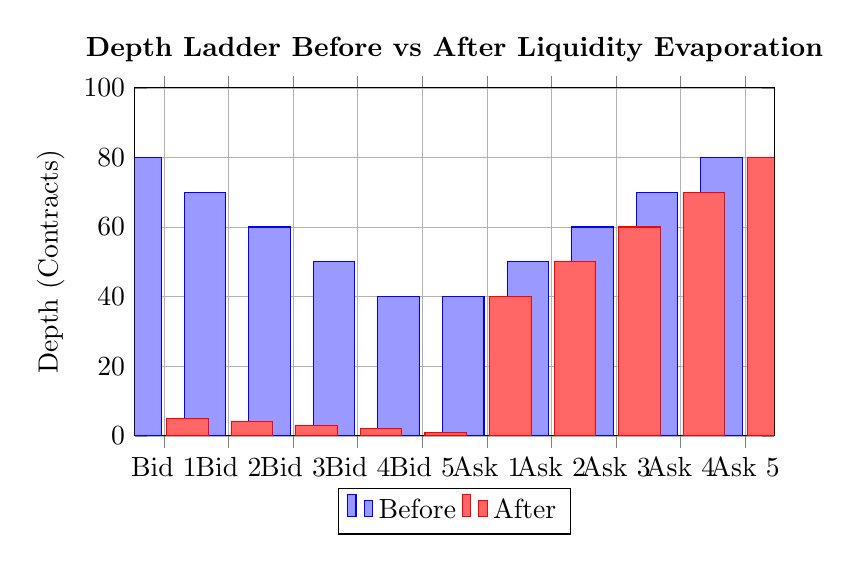
\begin{tikzpicture}
    \begin{axis}[
      ybar,
      bar width=15pt,
      width=0.8\textwidth,
      height=6cm,
      ymin=0,
      ymax=100,
      xtick=data,
      xticklabels={
        Bid 1, Bid 2, Bid 3, Bid 4, Bid 5, Ask 1, Ask 2, Ask 3, Ask 4, Ask 5
      },
      xlabel={Order Book Levels},
      ylabel={Depth (Contracts)},
      grid=both,
      grid style={line width=.1pt, draw=gray!20},
      major grid style={line width=.2pt, draw=gray!60},
      enlarge x limits=0.05,
      title={\textbf{Depth Ladder Before vs After Liquidity Evaporation}},
      legend style={at={(0.5,-0.15)}, anchor=north, legend columns=2}
    ]

    % Depth BEFORE evaporation
    \addplot+[fill=blue!40!white] coordinates {
      (0,80) (1,70) (2,60) (3,50) (4,40) (5,40) (6,50) (7,60) (8,70) (9,80)
    };

    % Depth AFTER evaporation (Bids collapse)
    \addplot+[fill=red!60!white] coordinates {
      (0,5) (1,4) (2,3) (3,2) (4,1) (5,40) (6,50) (7,60) (8,70) (9,80)
    };

    \legend{Before, After}

    \end{axis}
  \end{tikzpicture}
  \caption{Liquidity in the primary venue vanished: top five bids collapsed in seconds, leaving the book dangerously thin.}
\end{figure}

\medskip

David leaned in. “So we’re routing?”

“Yeah,” she said. “Model kicked us to synthetic.”

\begin{TechnicalSidebar}{Routing to Synthetic Liquidity}

  When Kayla says the model “kicked us to synthetic,” she’s referring to an automated execution strategy that 
  detects degraded conditions on the primary venue — in this case, an abrupt collapse in order book depth — 
  and reroutes the trade to an alternative execution path.

  \medskip
  
  \textbf{Synthetic liquidity} is constructed rather than naturally present. It may involve:

  \medskip

  \begin{itemize}
    \item Splitting orders across multiple venues with partial depth.
    \item Using correlated instruments (e.g., futures, ETFs, or options) to replicate exposure.
    \item Engaging internal crossing networks or dark pools where resting liquidity is not visible on the open book.
  \end{itemize}
  
  \medskip
  
  The model doesn’t “panic.” It observes a collapse in volume behind the top-of-book and recognizes that 
  routing to the lit market would create excessive slippage or signal risk. So it pivots — away from the 
  fragile, visible market, and toward a stitched-together execution pathway that mimics desired exposure 
  while minimizing footprint.
  
  \medskip
  
  This kind of behavior reflects \textbf{execution intelligence} — not just reacting to price, but adapting 
  to the structure and \textit{availability} of liquidity itself.
  
\end{TechnicalSidebar}
  

He looked up at the wallboard — aggregate execution volume had nearly tripled in the last 40 seconds.
“Is that all ours?”

She nodded. “London channel. Synthetic cleared. TRSs
\footnote{A \textbf{Total Return Swap (TRS)} is a financial contract where one party receives the total return (income 
plus capital gains) of an asset—like a stock or index—without actually owning it. Instead of buying the asset, they pay 
a fixed or floating rate and get exposure to its performance. It's a way to bet on price movements or earn yield without 
putting the asset on your balance sheet.}
and OTC
\footnote{\textbf{OTC} stands for \textbf{Over-the-Counter} — meaning trades that happen directly between parties, outside 
of formal exchanges like the NYSE. These deals are often private, less regulated, and tailored to the needs of the 
counterparties. While flexible, they can be harder to track and price compared to exchange-traded assets.}
look-throughs.”

David’s brow furrowed. “And latency?”

Kayla tapped the corner of her screen. “Spiked as we pivoted. London’s clearing, but there’s friction.”

\medskip

\begin{TechnicalSidebar}{Clearing Friction}

  Clearing friction refers to the \textbf{delay, cost, or operational resistance} that occurs when trades—especially 
  synthetic or over-the-counter (OTC) ones—are routed through clearinghouses or counterparties under stress.
 
  \medskip
  
  When Kayla says “London’s clearing, but there’s friction,” she means the systems are \textbf{accepting trades}, 
  but with signs of **stress or congestion**—either in settlement times, confirmation cycles, or collateral updates.

  \medskip
  
  \textbf{Common sources of clearing friction:}

  \medskip

  \begin{itemize}
    \item Latency between counterparties, often amplified across jurisdictions.
    \item Margin recalculations due to fast-moving underlying prices.
    \item Netting conflicts across synthetic layers (e.g., TRS offsetting vs. real inventory).
    \item Liquidity mismatches between executed volume and available credit lines.
  \end{itemize}
  
  \medskip
  
  \textbf{Why it matters:}  

  \medskip

  Friction isn’t just annoying—it’s structurally dangerous. In volatile moments, even a few seconds of delay in 
  confirmation or funding can cause:

  \medskip

  \begin{itemize}
    \item Execution throttles
    \item Forced hedging at wider spreads
    \item Cascading stop-outs due to margin lag
  \end{itemize}

  \medskip
  
  Clearing friction is often invisible until it breaks something. It doesn’t show up in price—it shows up in 
  \textit{timing}.  
  And in high-frequency structures, timing \textit{is} price.
  
\end{TechnicalSidebar}

\medskip

From the far side of the pit, a junior from quant ops shouted over.

“Someone just hit size on the back leg. Thirty mil notional. Full slip.”

\medskip

\begin{figure}[H]
  \centering
  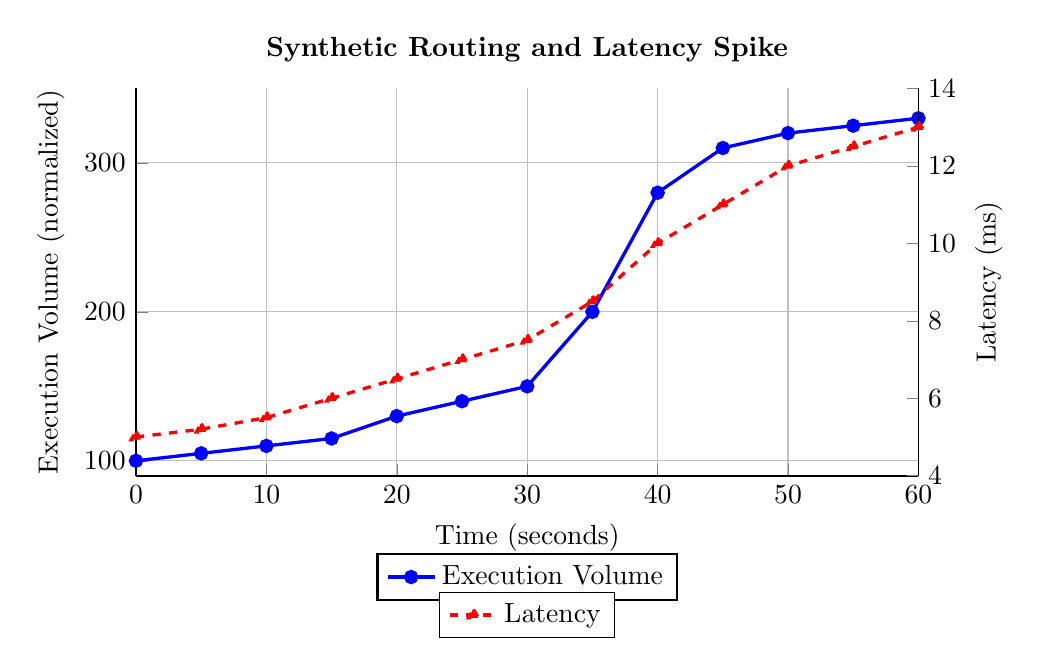
\begin{tikzpicture}
    \begin{axis}[
      width=0.95\textwidth,
      height=6.5cm,
      xlabel={Time (seconds)},
      ylabel={Execution Volume (normalized)},
      xmin=0, xmax=60,
      ymin=90, ymax=350,
      grid=both,
      thick,
      axis y line*=left,
      axis x line*=bottom,
      legend style={at={(0.5,-0.2)}, anchor=north, legend columns=2},
      title={\textbf{Synthetic Routing and Latency Spike}},
    ]
    \addplot[very thick, blue, mark=*] coordinates {
      (0,100)
      (5,105)
      (10,110)
      (15,115)
      (20,130)
      (25,140)
      (30,150)
      (35,200)
      (40,280)
      (45,310)
      (50,320)
      (55,325)
      (60,330)
    };
    \addlegendentry{Execution Volume}
    \end{axis}

    \begin{axis}[
      width=0.95\textwidth,
      height=6.5cm,
      xmin=0, xmax=60,
      ymin=4, ymax=14,
      ylabel={Latency (ms)},
      axis y line*=right,
      axis x line=none,
      ytick={4,6,8,10,12,14},
      legend style={at={(0.5,-0.3)}, anchor=north, legend columns=2},
    ]
    \addplot[very thick, red, dashed, mark=triangle*] coordinates {
      (0,5)
      (5,5.2)
      (10,5.5)
      (15,6)
      (20,6.5)
      (25,7)
      (30,7.5)
      (35,8.5)
      (40,10)
      (45,11)
      (50,12)
      (55,12.5)
      (60,13)
    };
    \addlegendentry{Latency}
    \end{axis}
  \end{tikzpicture}
  \caption{Execution volume spiked as synthetic routing was triggered. Latency rose simultaneously, reflecting clearing frictions.}
\end{figure}

\medskip

David didn’t respond. He was already moving.

He stopped at the master terminal, toggled the trace overlay. The execution route had redrawn itself — not gradually, 
but all at once, a perfect right-angle jump away from the primary venue into synthetic space.

There was no alert.
No error.
Just a clean reroute — and a tripling of volume.

He exhaled slowly.

“Tell London to watch their slip buffers,” he said. “And flag me if spread volatility crosses threshold. I want eyes on 
every delta over 2 mil.”

\medskip

\begin{TechnicalSidebar}{What’s Spread Volatility?}

  \textbf{Spread volatility} measures how much the bid-ask spread — the gap between the highest price buyers are willing 
  to pay (bid) and the lowest price sellers will accept (ask) — fluctuates over time.
  
  \medskip
  
  In stable markets, spreads are tight and steady.  
  In stressed markets, spreads widen and bounce — often erratically.
  
  \medskip
  
  Why it matters:

  \medskip
  
  \begin{itemize}
    \item \textbf{Execution Risk:} A volatile spread means trade execution costs become unpredictable. You might think 
    you're crossing a 2bp spread — and suddenly it's 14.
    
    \item \textbf{Slippage:} When spreads move during routing or order execution, you get worse prices than modeled. 
    This is called \textit{slippage}, and it adds hidden cost.
    
    \item \textbf{Signal Noise:} High spread volatility can mimic panic or create false market signals, especially in 
    algorithmic models that interpret microstructure.
  
    \item \textbf{Synthetic Routing Sensitivity:} When spreads swing too fast, synthetic channels might misfire — mistaking 
    noise for opportunity.
  \end{itemize}
  
  \medskip
  
  In this context, David’s instruction to flag threshold-crossing spread volatility is a preemptive risk control — looking for signs of structural instability before the numbers fully catch up.
  
\end{TechnicalSidebar}

\medskip


Kayla nodded without turning.

He glanced at the ladder again.
Still dry.

Synthetic trades were printing, but they weren’t behaving like mirrors. They were too willing.

David frowned.

He'd seen this before as a case study.
It wasn’t panic.
It was extraction.



One morning in Chicago 2016, a biotech company had posted disappointing trial results. 
It was nothing catastrophic. It was just enough to spook the 
retail crowd. The stock dropped 5\% in the first few minutes. It was predictable and expected; so, the models adjusted 
accordingly.

But then something strange happened.

The bids started vanishing across the sector. It was not all at once, and it was not visibly. It was like fog receding. 
The depth behind the price thinned, and spreads widened.

A handful of firms were suddenly active, quietly buying at wide spreads, 
and scooping up liquidity that wasn’t supposed to be available. They weren’t fleeing the market.

They were harvesting it.

\textit{It was like watching a fire drill staged by the people who knew there wasn’t really a fire.}

They’d let the rumor run just long enough. They let the weak hands sell. They let the algos trigger stop-losses.
Then they stepped in and calmly, methodically, and predatorily picked through the wreckage.

On that day, David had watched from his desk, frozen in that strange awe you feel when you realize the thing falling apart was never 
meant to stay intact. It was bait.

That was the day he learned the difference.

Panic is disorder. Panic is  Emotional. And panic is unscripted.
But extraction is choreographed. Extraction is intentional. And it
profits from how others react when they do.

And what he was seeing now --— the blank depth ladder, the vanishing bids, and the quiet shift to synthetic routing —-- 
wasn’t a crisis.

It was a vacuum being created on purpose.

Like someone had sucked the oxygen out of the room, just to watch who gasped first.

\textit{This wasn’t a glitch. This was a harvest.}

He looked back at Kayla’s screen. The top five bids were gone. The rest of the book was too shallow to trust.

There were no fire alarms, or chaos.
There was just silence and footprints.

They weren’t in the wrong place.
They were in someone else’s trap.

And they were the ones bleeding.

\medskip

\begin{figure}[H]
  \centering
  \begin{tikzpicture}[
      node/.style={circle, draw, thick, minimum size=2cm, align=center, font=\small, fill=gray!10},
      arrow/.style={->, very thick, >=latex},
      dashedarrow/.style={->, very thick, dashed, >=latex},
      annotation/.style={font=\footnotesize},
      legendbox/.style={draw, fill=white, rounded corners, thick, align=left, font=\footnotesize, text width=5cm},
      actorlegend/.style={draw, fill=gray!5, rounded corners, thick, align=left, font=\footnotesize, text width=5cm}
    ]

    % Nodes
    \node[node, fill=red!10] (panic) at (0,0) {Panicking\\Traders};
    \node[node, fill=green!15] (extractor) at (6,2) {Extractors\\(Informed)};
    \node[node, fill=blue!10] (extracted) at (6,-2) {Extraction\\Targets};

    % Curved solid arrows (value/risk flow)
    \draw[arrow] (panic) .. controls +(2,1.5) and +(-2,0.5) .. (extractor);
    \draw[arrow] (extracted) .. controls +(2,-1.5) and +(-2,-0.5) .. (extractor);

    % Curved dashed arrows (influence/signal)
    \draw[dashedarrow] (extractor) .. controls +(-2,1) and +(2,1.5) .. (panic);
    \draw[dashedarrow] (extractor) .. controls +(-2,-1) and +(2,-1.5) .. (extracted);

    % Arrow legend (top right)
    \node[legendbox, right=2cm of extractor] (legend1) {
      \textbf{Arrow Legend} \\[0.5em]
      \textbf{→} Solid Arrows: Flow of Liquidity, Risk, and Value \\
      \textbf{⇢} Dashed Arrows: Indirect Influence or Signaling
    };

    % Actor legend (below arrow legend)
    \node[actorlegend, below=0.5cm of legend1] (legend2) {
      \textbf{Actor Legend} \\[0.5em]
      \textbf{Panicking Traders (Red)}: Retail traders, reactive algos, momentum funds caught in the move. \\[0.5em]
      \textbf{Extractors (Green)}: Informed players — HFT firms, institutional desks, or insiders exploiting the event. \\[0.5em]
      \textbf{Extraction Targets (Blue)}: Passive funds, stale quote providers, market makers unable to adjust in time.
    };

  \end{tikzpicture}
  \caption{Visualizing market roles during a structured extraction event. Two legends separate directional logic from actor identity.}
\end{figure}

\medskip


David didn’t say anything.

Everyone around him was either moving too fast or freezing up — eyes locked on depth ladders, correlation spreads, synthetic hedges that were unraveling faster than ops could route. Voices rising, risk boards flashing, alerts pinging without hierarchy.

But he just stood there.

Still.

Watching it unfold like a machine he already knew how to take apart.

Because he’d seen this before — not just in the models, but in the shape of the failure.

This wasn’t panic. Not really. It was choreography gone recursive. A snake eating its own tail.

Arcadia was bleeding — and they didn’t even realize it was their own blade.

\textit{We trained the models to exploit weakness. Now someone’s exploiting the models.}

It was the perfect loop. The predator had become visible. Their footprint was traceable. And someone, somewhere, had reverse-engineered their execution logic just well enough to tilt the floor beneath their feet.

It wasn’t sabotage. It didn’t need to be.

\textit{Just wait. Let our models overcommit. Let our own overconfidence fill the book. Then hit it from the other side.}

That was the genius of it.
Whoever was behind it didn’t need to be faster. They just needed to be patient.

And now Arcadia — the firm that once made markets jump by blinking — was gasping like retail. Caught in the very 
structure it had once mastered.

David saw the humor in it. The kind that only clicks when you’re standing at the edge of something large and 
expensive and watching it break exactly the way you warned it might.

\textit{We were the extractor. Now we’re the signal.}

And nobody had time for a lecture. Not now.

No one wanted to hear about structural irony, or how meta-predictability becomes fragility. No one wanted to 
discuss behavioral mirroring or second-order game theory. They just wanted him to fix it.

\textbf{Because now it was his job to stop it.}

Not to outtrade it. Not to outshout it.

But to \textit{break the loop}.

Before the next cascade started.

Before someone else got clever enough to harvest the rest.

\medskip

\begin{figure}[H]
  \centering
  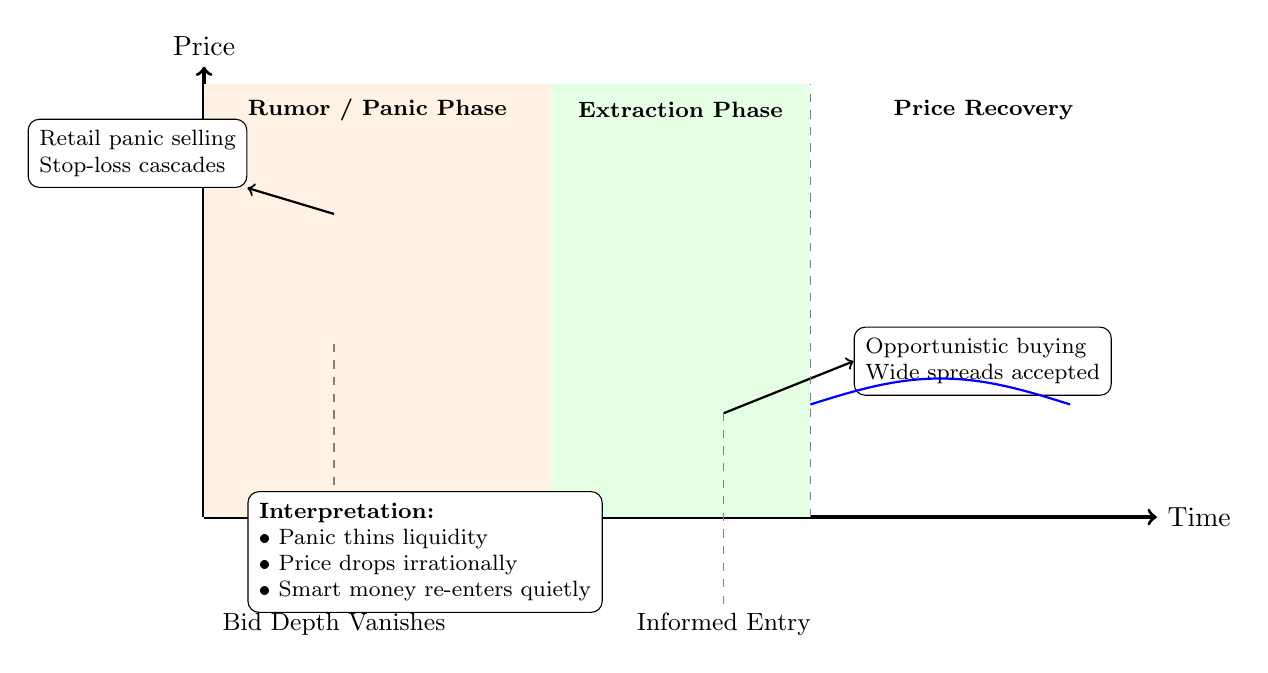
\begin{tikzpicture}[
      scale=1.1,
      axis/.style={very thick,->},
      label/.style={font=\footnotesize},
      dashedline/.style={gray, dashed},
      annotation/.style={draw=black, fill=white, font=\footnotesize, align=left, rounded corners, inner sep=4pt}
    ]

    % Axes
    \draw[axis] (0,0) -- (11,0) node[right] {Time};
    \draw[axis] (0,0) -- (0,5.2) node[above] {Price};

    % Price drop curve
    \draw[thick, blue, smooth, samples=100, domain=0:4] plot(\x,{4 - 0.3*\x*\x});
    \draw[thick, blue, smooth, samples=100, domain=4:7] plot(\x,{0.2 + 0.05*(\x - 4)^2});

    % Rumor zone
    \fill[orange!10] (0,0) rectangle (4,5);
    \node[label] at (2,4.7) {\textbf{Rumor / Panic Phase}};

    % Extraction zone
    \fill[green!10] (4,0) rectangle (7,5);
    \node[label] at (5.5,4.7) {\textbf{Extraction Phase}};

    % Depth Ladder Illustration
    \draw[dashedline] (1.5,2) -- (1.5,-1);
    \node[below] at (1.5,-1) {\small Bid Depth Vanishes};

    \draw[dashedline] (6,1.2) -- (6,-1);
    \node[below] at (6,-1) {\small Informed Entry};

    % Arrows and Annotations
    \draw[->, thick] (1.5,3.5) -- (0.5,3.8);
    \node[annotation, above left] at (0.5,3.8) {
      Retail panic selling \\
      Stop-loss cascades
    };

    \draw[->, thick] (6,1.2) -- (7.5,1.8);
    \node[annotation, right] at (7.5,1.8) {
      Opportunistic buying \\
      Wide spreads accepted
    };

    % Market resumes
    \draw[dashedline] (7,0) -- (7,5);
    \node[label] at (9,4.7) {\textbf{Price Recovery}};

    \draw[thick, blue, smooth, samples=100, domain=7:10] plot(\x,{1.3 + 0.3*sin((\x-7)*180/3)});

    % Legend box
    \node[annotation, below right] at (0.5,0.3) {
      \textbf{Interpretation:} \\
      \textbullet~Panic thins liquidity \\
      \textbullet~Price drops irrationally \\
      \textbullet~Smart money re-enters quietly
    };

  \end{tikzpicture}
  \caption{Price action and liquidity behavior during engineered extraction: a panic event seeded by rumor, followed by informed re-entry.}
\end{figure}

\medskip

\medskip

\begin{HistoricalSidebar}{Leverage via Synthetic Exposure}

Total return swaps (TRS) and other synthetic instruments allow firms to gain economic exposure to assets 
without owning them.

\medskip

They’re efficient but obscure true exposure — especially when fallback logic routes multiple desks through the same 
synthetic pipe.

\medskip

That’s how Archegos blew through its caps across five banks, and no one knew until margin calls hit.

\end{HistoricalSidebar}

\subsection{Threshold Breach with No Flag (08:24 AM)} 

\subsubsection{Too Fast to Brake}

The lights in the war room were low, but the screens burned hot — sixteen terminals in a crescent arc, each bleeding red in its own rhythm.

David stood alone at the center console, collar loose, tie gone, two days past a full night’s sleep.

“Pull latest NAV delta,” he muttered.

The terminal chirped.
NAV down 6\%.
(\$750 million).

He stared. That wasn’t drift. That was hemorrhage.

He toggled the circuit overlay — the threshold logic was live, limiters engaged. But the drawdown was still compounding.

“That’s too much,” he said, mostly to himself. “The model’s not supposed to breach 4\% without circuit deceleration.”

\medskip

\begin{TechnicalSidebar}{What is Circuit Deceleration?}

  \textbf{Circuit deceleration} is a built-in risk mechanism used in automated trading systems to prevent runaway losses 
  during unexpected market moves.
  
  \medskip
  
  Just as traditional exchanges have \textit{circuit breakers} that halt trading when price moves exceed a certain threshold, 
  circuit deceleration acts as a \textit{soft brake} — it doesn't stop trading entirely, but slows it down when certain 
  limits are crossed.
  
  \medskip
  
  In practice, this means:

  \medskip

  \begin{itemize}
    \item Reducing order size.
    \item Increasing wait time between executions.
    \item Temporarily narrowing the range of allowed trades.
  \end{itemize}
  
  \medskip

  The goal is to avoid amplifying losses through momentum or liquidity slippage. 
  
  \medskip
  
  In David’s case, the model was supposed to throttle down when Net Asset Value (NAV) dropped more than 4\%. But it didn’t — 
  and the losses kept accelerating. That’s what made it so dangerous: the guardrails were technically active, but something 
  had disabled their grip.

\end{TechnicalSidebar}

\medskip

His hands moved fast, muscle memory over keyboard:
\texttt{fetch: threshold.logs.execution-level}

The heatmap flickered. Execution weights were peaking in synthetic — but without fallback deferrals. No redistribution.
No load balancing.

\medskip

\begin{figure}[H]
  \centering
  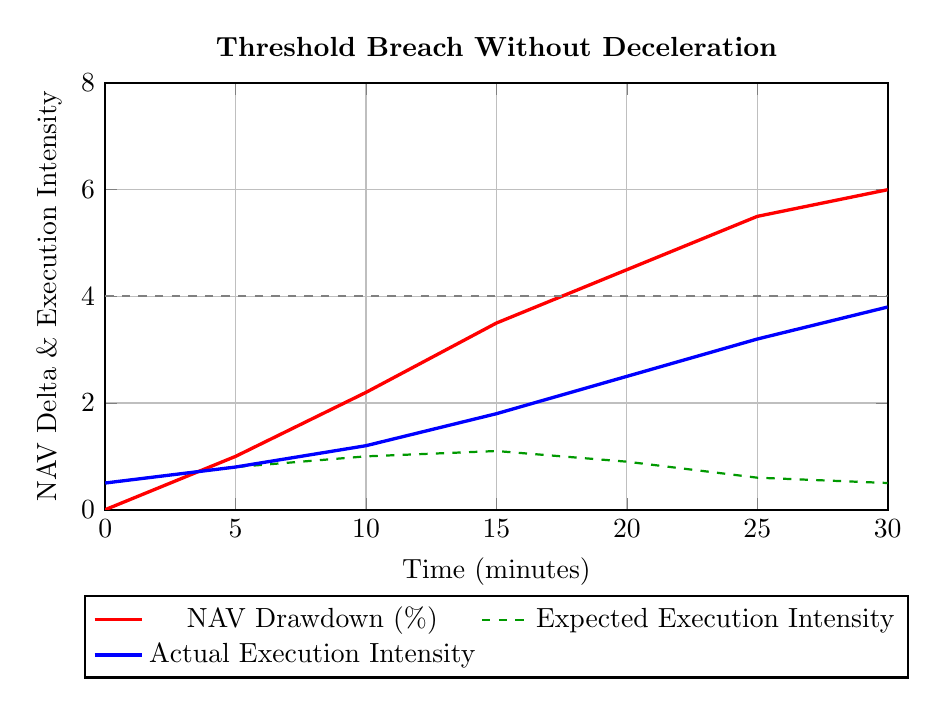
\begin{tikzpicture}
    \begin{axis}[
      width=0.95\textwidth,
      height=7cm,
      xlabel={Time (minutes)},
      ylabel={NAV Delta \& Execution Intensity},
      xmin=0, xmax=30,
      ymin=0, ymax=8,
      legend style={at={(0.5,-0.2)}, anchor=north, legend columns=2},
      grid=both,
      thick,
      title={\textbf{Threshold Breach Without Deceleration}},
    ]
    
    % NAV Drawdown
    \addplot[very thick, red] coordinates {
      (0, 0)
      (5, 1.0)
      (10, 2.2)
      (15, 3.5)
      (20, 4.5)
      (25, 5.5)
      (30, 6.0)
    };
    \addlegendentry{NAV Drawdown (\%)}

    % Circuit Deceleration Trigger (should reduce intensity)
    \addplot[dashed, green!60!black, thick] coordinates {
      (0, 0.5)
      (5, 0.8)
      (10, 1.0)
      (15, 1.1)
      (20, 0.9)
      (25, 0.6)
      (30, 0.5)
    };
    \addlegendentry{Expected Execution Intensity}

    % Actual Execution Intensity (still rising)
    \addplot[very thick, blue] coordinates {
      (0, 0.5)
      (5, 0.8)
      (10, 1.2)
      (15, 1.8)
      (20, 2.5)
      (25, 3.2)
      (30, 3.8)
    };
    \addlegendentry{Actual Execution Intensity}

    % Threshold Line
    \draw[dashed, gray] (axis cs:0,4) -- (axis cs:30,4);
    \node at (axis cs:30,4.1) [above right, font=\small] {4\% Deceleration Threshold};

    \end{axis}
  \end{tikzpicture}
  \caption{NAV drawdown breached the 4\% threshold. Circuit deceleration logic was live, but execution intensity continued climbing — indicating system failure to engage safeguards.}
\end{figure}

\medskip

He hit the comms line.

“Risk, this is David. We’re showing a \$750 mil draw and circuit limits aren’t firing. Confirm threshold matrix 
and escalation tree.”

Silence.

He waited.

Nothing.

The call auto-looped to voicemail.

He hit it again, this time direct to Julia’s line in Risk. Nothing.

\medskip

\begin{HistoricalSidebar}{The Separation of Risk}

  In the wake of major financial collapses — from \textit{Barings Bank} to \textit{Lehman Brothers} — regulators and 
  institutions began rethinking the structure of risk oversight.
  
  \medskip
  
  One key reform: \textbf{segregation of risk teams} from trading desks.
  
  \medskip
  
  Originally, risk was embedded — sometimes literally sitting beside traders. That made for speed, but blurred lines. 
  Risk managers would flag exposure in real-time, but social dynamics often muted escalation. In some cases, “risk” 
  became more concerned with smoothing variance than preventing it.
  
  \medskip
  
  After the 2008 crisis, a shift began:

  \medskip

  \begin{itemize}
    \item Risk was restructured as a separate reporting chain — typically under the CFO or Chief Risk Officer.
    \item Geographic and physical separation followed: off-floor offices, remote monitoring, firewalled access.
    \item Tools moved toward automation: dashboards, alerts, circuit thresholds, escalation matrices.
  \end{itemize}
  
  \medskip
  
  The goal: independence and objectivity.

  \medskip
  
  But the tradeoff was clear — \textbf{latency of judgment}. By the time a system flagged a breach and escalated it 
  to a risk officer — possibly remote, possibly asleep — the loss had already metastasized.
  
  \medskip
  
  In David’s case, this delay was existential. The floor was melting, but risk had been abstracted — away from the 
  room, away from the rhythm, away from the trade.
  
\end{HistoricalSidebar}

\medskip

\subsubsection{The Compliance Illusion}

He stood there, listening to the quiet hiss of the line, the click of trades printing downstream, and the faint hum of 
fans behind the rack servers.

Then, flatly: “No answer.”

From across the room, Kayla looked up.
“They’re not in the pit,” she said. “They were pushed remote overnight due to a server compliance patch.”

David’s jaw tensed.

David didn’t respond right away.

The words hung in the air --— \textit{pushed remote overnight} --— as if they were harmless. As if they were procedural. 
As if it was just another IT memo that had passed through five inboxes and picked up six approvals.

But his mind was already pulling threads.

David didn’t move. He just stared at the screen, watching the indicators stay green while the world 
beneath them frayed.

They’d killed local ops to pass compliance review. That much was already obvious.

Somewhere, a project manager had checked a box that said “remote failover validated,” and nobody had asked 
what that actually meant at 8:57 AM with liquidity unraveling.

``Did we even test the kill-switch handoff, properly?'' he wondered. 

His mind retraced the last deployment cycle where they rushed to meet internal audit. The one where they 
skipped full-path latency tests because the VP of Regulatory Strategy needed a bullet point that said, 
\textit{“Regionally mirrored with failover readiness.”}

But it wasn’t readiness. It was narrative.

Was the failover even flagged in the deployment log? Or had it slipped in through one of the silent pushes 
that didn’t go through full review?

He already knew the answer. They’d been warned not to “create noise” ahead of earnings week. That meant no 
change requests. No escalations. No alarms.

And so engineering did what it always did under pressure: it gritted its teeth and made the green lights 
blink.

``Did we properly validate the latency budget under stress?'' he said to himself and the thought landed cold. 
He doubted it. The numbers had looked too clean. The numbers looked too synthetic.

He exhaled through his nose.

They wanted zero-downtime ops.  
They wanted “streamlined coverage.”  
They wanted fallback on paper and throughput in the cloud.  

But they didn’t want to pay for it.

David clenched his jaw.

The truth was brutal in its simplicity: the system hadn’t broken.  
It had done exactly what it was designed to do:  
minimize noise, preserve optics, and delay escalation.

Now the risk team was unreachable.  
The fallback loop had no owner.  
And the synthetic desk was melting through its buffers.

David scanned the console again.

Green lights.  
Silent logs.  
And a compliance sheet that would pass review tomorrow.

He whispered, barely audible, “But the floor’s on fire.”

And still no one answered.

He knew what it meant: \textbf{No one was at the controls.}

The algos were live, the flow was real,  
and the one person who could stop the bleeding had been virtualized out of relevance.

He had seen this before in postmortems.

\begin{quote}
\textit{Every failure starts with a missing name on a call sheet.} 
\textit{Every meltdown begins with someone thinking fallback coverage meant actual coverage.}
\end{quote}

It wasn’t malice. And It was design drift.  
It was a thousand small choices --- none catastrophic alone --- but aligned in just the right (or wrong) 
way to remove accountability in real time.

\begin{quote}
\textit{They think ``automated'' means safe. But all it means is faster.} 
\textit{Faster execution. Faster contagion. Faster loss.}
\end{quote}

He took a breath, shallow and stale.

\begin{quote}
\textit{No human in the loop. Just logs. Just green lights. Just blind systems doing exactly what they were told.} 
\textit{Even if what they were told made no sense anymore.}
\end{quote}

Across the floor, someone coughed. The sound echoed like a fire alarm in a padded cell.

David turned back to the console.

``Okay,'' he thought. ``Then we become the loop.''

“Patch or not, someone should’ve flagged this. The circuit breaker is green, but the floor’s melting.”

He glanced at the execution wallboard. Synthetic volumes were surging, but the slip buffers weren’t scaling. They 
were still using Friday’s volatility model.

He exhaled, slowly. “Okay. We do this the hard way.”

He turned back to his terminal.

“Override auto-throttle. Route audit. Flag anything above \$10 mil notional and reroute to soft-ice. And find 
me a human in Risk.”

\medskip

\begin{HistoricalSidebar}{What is Soft-Ice?}

  \textbf{Soft-ice} is a tactical risk containment strategy used in high-frequency and algorithmic trading 
  environments. It’s not a full halt — it’s a controlled slowdown.
  
  \medskip
  
  Think of it as the financial equivalent of tapping the brakes without pulling the handbrake.
  
  \medskip
  
  The term emerged post-Flash Crash (2010), when firms realized that \textbf{hard circuit breakers} — like 
  exchange-level trade halts — often came too late or were too blunt. What was needed was a way to:

  \medskip

  \begin{itemize}
    \item Triage abnormal flow,
    \item Quarantine large or suspicious trades,
    \item And give humans a few precious seconds to intervene.
  \end{itemize}
  
  \medskip
  
  A typical \textbf{soft-ice routine} involves:

  \medskip

  \begin{itemize}
    \item \textit{Flagging trades} over a notional threshold (e.g., \$10 million),
    \item \textit{Re-routing them} to non-aggressive execution pools,
    \item \textit{Introducing delay buffers} to pace their impact,
    \item And optionally, \textit{requiring manual release}.
  \end{itemize}
  
  \medskip
  
  It’s not about stopping the machine. It’s about slowing it just enough to regain control — to shift from 
  reflex to awareness.
  
  \medskip
  
  In David’s case, “soft-ice” wasn’t a protocol. It was a last resort — invoked when the model failed, the 
  guardrails slipped, and no one in Risk picked up the phone.
  
\end{HistoricalSidebar}

\medskip


Kayla nodded.

“On it.”

The room, still dim, felt smaller now. The kind of small that means you're alone in something that used to be shared.


  

\subsection{Manual Pause Failure and Synthetic Override (08:28 AM)}

The lights in the war room were still low, but the tempo had changed. The air felt tighter — like a room that's 
been holding its breath too long.

David leaned over his terminal. His shirt was damp at the collar. The sleeve was rolled high enough to show the 
scar on his forearm — a burn from his first month on the desk, back when the servers still ran hot enough to brand you.

\texttt{fetch: nav.delta.current}

The response blinked in yellow, then red.

\textbf{NAV down 12\%.}
\textbf{(\$1.5 billion)}

He didn’t speak at first. Just stared.
Twelve percent wasn’t drawdown. That was freefall.

He keyed the override.
\texttt{manual.pause.execution.all}

Nothing.

He tried again, fingers slower this time, deliberate.
\texttt{manual.pause.execution.all}

The screen chirped.

\texttt{[Error: Local command blocked. Routing active — Arcadia.Synthetic.LDN]}

He whispered, “You’ve got to be kidding me.”
Then louder: “Kayla. Why the hell is London still routing?”

She spun from her desk. “I thought you killed the synthetic pipe.”

“I did.” He pointed at his terminal. “But the model’s not executing local. It’s live in London. And it’s not listening.”

She blinked, then checked the route audit feed. Her voice was flat. “Arcadia desk re-registered last night — backup 
routing from the LDN cluster.”

“No confirmation?”

“Nothing was flagged.”

David swore under his breath.

He stood, pacing the crescent of terminals like someone walking a minefield in real time.

“We’re hemorrhaging into synthetic,” he said. “And we’re not holding the keys.”

From across the room, Tom from infra looked up. “Want me to hard-kill London?”

David paused. The question was tactical. The implications weren’t.

He exhaled. “No. Not yet. We don’t know what they’re holding. Pull a shadow log. Full trace. And lock out anything 
over \$5 mil until I say otherwise.”

He sat again. Slowly.

And then, quietly: “We built a model smart enough to reroute around us. Now we’re just passengers.”

NAV down 12\% (\$1.5 billion).

David issues a manual pause command from his terminal.

It fails — the model isn’t executing locally. It’s routing through Arcadia’s synthetic desk in London.

\medskip

\begin{figure}[H]
  \centering
  \begin{tikzpicture}[
    node distance=2.5cm and 3.5cm,
    box/.style={draw, thick, rectangle, rounded corners, minimum width=3.5cm, minimum height=1.2cm, align=center},
    arrow/.style={->, thick},
    failed/.style={->, thick, red, dashed},
    reroute/.style={->, thick, blue, dashed}
  ]

  % Nodes
  \node[box, fill=gray!10] (model) {Trading Model\\(Local Node)};
  \node[box, fill=green!10, right=of model] (primary) {Primary Venue\\(Exchange)};
  \node[box, fill=blue!10, below=of primary, xshift=1.5cm] (arcadia) {Arcadia\\Synthetic Desk (LDN)};
  \node[box, fill=red!10, below=of model] (manual) {Manual Pause\\Command};

  % Arrows
  \draw[arrow] (model) -- node[above] {Normal Route} (primary);
  \draw[reroute] (model) -- node[right, font=\small] {Synthetic Reroute} (arcadia);
  \draw[failed] (manual) -- node[right, font=\small] {Blocked} (model);

  % Annotations
  \node at ($(model)!0.5!(primary)+(0,1.1)$) [font=\small] {Initial execution path};
  \node at ($(model)!0.5!(arcadia)+(-1.7,-0.3)$) [font=\small, rotate=25] {Fallback route activated};
  \node at ($(manual)!0.5!(model)+(-1.4,-0.3)$) [font=\small, rotate=25, text=red!70!black] {Override rejected};

  \end{tikzpicture}
  \caption{Execution path rerouted from primary venue to Arcadia’s synthetic desk in London. Manual pause command blocked due to remote override.}
\end{figure}

\medskip

\begin{HistoricalSidebar}{Arcadia’s Synthetic Desk}

  \textbf{Arcadia’s Synthetic Desk} isn’t a place. It’s a mechanism — a routing layer of execution logic designed to simulate liquidity across fragmented venues, without relying on any single one.
  
  \medskip
  
  Originally developed to handle after-hours execution in thin markets, synthetic desks evolved into high-frequency liquidity engines. Instead of sending orders directly to a single exchange, they decompose, mirror, and redistribute trades across internal books, dark pools, and algorithmic clearing channels — all while maintaining a unified execution surface.
  
  \medskip
  
  \textbf{Why use it?}
  \begin{itemize}
    \item To avoid market impact on large trades.
    \item To obfuscate size, intention, and direction from counterparties.
    \item To route around slippage and latency on overloaded venues.
  \end{itemize}
  
  \medskip
  
  \textbf{Why is it dangerous?}
  
  Because once a system is rerouted through synthetic, local controls often lose priority. Manual throttles, visibility on internal slippage, and even circuit deceleration can be bypassed — especially when routed across jurisdictions (like London). Arcadia’s synthetic layer is fast, adaptive, and capital-efficient — but it was never meant to act as a failsafe.
  
  \medskip
  
  In David’s case, the model rerouted into Arcadia’s synthetic desk without error — and without escalation. The fallback wasn’t broken.
  
  It was working as designed.
  
\end{HistoricalSidebar}

\medskip

\begin{tcolorbox}[title=Fragmented Risk Systems, colback=gray!5, colframe=black]
Pre-trade risk, post-trade margining, and synthetic credit exposure are often handled by different systems — and teams — with asynchronous data refresh cycles.\\
A misconfigured cap in one system won’t alert the others unless explicitly bridged.\\
Knight Capital and Archegos both blew up in that space between domains.
\end{tcolorbox}


\subsection{The Illusion of Fallbacks (08:33 AM)} 
The fluorescents above the trading floor had dimmed to half-light — not for mood, but because someone had 
killed the overheads three hours ago to make the screen glare tolerable. The room smelled like warm plastic and stale caffeine. Terminals flickered. Execution ladders scrolled. But no one was talking.

David stood near the elevated console, one hand gripping the edge of the desk like it could keep him tethered. On-screen:
NAV delta: –18.2\%
Loss: \$2.25 billion.

He didn’t blink.

“Three fallbacks,” Kayla said behind him, her voice thin. “Primary routed to Synthetic. Synthetic spilled into TRS. 
TRS cleared through OTC overlay.”

“And nobody flagged?” David didn’t raise his voice.

“Each route assumed the one behind it was safe,” she said. “Classic fallback loop. No final owner.”

\begin{TechnicalSidebar}{Fallback Loops in Trading Systems}

  Fallbacks are intended as a safety mechanism — a chain of contingency routes triggered when the primary strategy 
  or execution path fails. But in complex, multi-layered systems, these safeguards can become sources of latent 
  fragility.

  \medskip
  
  A \textbf{fallback loop} occurs when each layer in a multi-route execution strategy assumes the downstream path has 
  been vetted and is fail-safe. In practice, this can lead to cascading delegation without ownership:

  \medskip

  \begin{itemize}
    \item \textbf{Primary} fails → routes to \textbf{Synthetic instrument}
    \item \textbf{Synthetic} hits limit → routes to \textbf{Total Return Swap (TRS)}
    \item \textbf{TRS} exceeds margin → auto-clears through \textbf{OTC overlay}
  \end{itemize}

  \medskip
  
  Each handoff assumes the next has controls. None verify the total exposure impact. The result is a hidden amplification 
  path: a feedback spiral where risk compounds rather than disperses.

  \medskip
  
  \textbf{Key failure mode:} No single system or team has complete visibility. When the fallback design lacks an 
  explicit \textit{terminal authority} or escalation flag, failure becomes silently recursive, and total.

  \medskip
  
  \textit{Symptoms of fallback loop risk:}

  \medskip

  \begin{itemize}
    \item Execution spans multiple asset classes with no common ledger
    \item Auto-routing rules cross desks or jurisdictions
    \item Margin offsets or hedges rely on inferred pricing assumptions
    \item Alerts are suppressed by assuming they were acknowledged upstream
  \end{itemize}

  \medskip
  
  \textbf{Lesson:} Redundancy without coordination is not resilience. It's just another route to system-wide opacity.

\end{TechnicalSidebar}

David’s jaw clicked.

He toggled his headset and hit the direct line. “Arcadia London — trading desk.”

A pause. A tone. Then a filtered voice.

\textbf{“Operations desk, London. Please hold.”}

\begin{HistoricalSidebar}{What is the Operations Desk — and Why Is It Separate from Risk?}

  The \textbf{Operations Desk} — often shortened to “Ops” — is the silent infrastructure of finance.  
  Historically, it evolved from back-office bookkeeping, responsible for trade settlements, reconciliations, 
  and counterparty clearing.  
  Today, it handles the \textit{plumbing} of modern markets: routing confirmations, managing post-trade events, 
  and ensuring that millions of automated transactions don't crash into regulatory walls.
  
  \medskip
  
  The reason it’s distinct from Risk is \textbf{functional separation}:

  \medskip
  
  \begin{itemize}
    \item \textbf{Risk} asks: “\textit{Should we do this?} What happens if it fails?”
    \item \textbf{Operations} asks: “\textit{How do we do this?} And who gets notified if it breaks?”
  \end{itemize}
  
  \medskip
  
  After the financial crises of the 2000s, regulators pushed for stricter firewalls between trading, risk management, 
  and post-trade operations — partly to avoid internal conflicts of interest, and partly to keep audit trails clean.  
  But in doing so, they also created \textit{institutional blind spots}.
  
  \medskip
  
  In a fallback cascade like David's, each system routed cleanly.  
  But no single desk had visibility into the full sequence — Risk saw the limits, Ops saw the flows,  
  and no one stitched the two together until it was too late.
  
\end{HistoricalSidebar}
  

He glanced at Kayla.

“They routed me to Ops.”

“Not risk?”

“Nope.”

\textbf{“Arcadia Ops. This is Sarah.”}

David spoke clearly. “Sarah — this is David Morales. You’re downstream of a triple-route model. NAV just crossed 
minus eighteen percent. I need to know if you’re aware.”

There was a rustle of paper, then a pause.

\textbf{“We’re triaging. Synthetic latency spiked after the 4:20 block. TRS cleanup lagged. There’s backflow 
on the OTC overlay.”}

David exhaled. “And risk escalation?”

\textbf{“Still waiting on threshold confirmation. Our dashboard’s green, but the trade footprints 
don’t match the logs.”}

He muted the call, turned to Kayla.

“They’re flying blind.”

She didn’t answer.

From the far end of the room, a junior quant muttered, “Wasn’t this supposed to be the safest route?”

David didn’t look up. His eyes were still fixed on the screen.

“Every fallback thinks it’s the last one,” he said. “Until the floor disappears beneath it.”

\medskip

\begin{TechnicalSidebar}{What is Fallback Logic?}

  \textbf{Fallback logic} is a built-in contingency system used in algorithmic trading architectures.  
  When a trade route or execution venue becomes unavailable — due to latency, slippage, illiquidity, or outright failure —  
  the model automatically redirects orders through an alternative path.

  \medskip

  The idea is redundancy:  
  If Exchange A goes dark, use Exchange B.  
  If Exchange B starts slipping, try the synthetic route.  
  If synthetic routes saturate, pivot to OTC or dark pools.

  \medskip

  But the danger of fallback logic isn’t failure — it’s \textit{false safety}.

  \medskip

  Each fallback assumes the previous risk has been mitigated.  
  And in a cascading stress scenario, every system downstream inherits a deeper exposure — without full context.  

  \medskip

  In David’s case, the model had passed through three fallback layers.  
  Each one routed cleanly — but none raised the flag.  
  Why? Because each assumed the last one had already done so.

  \medskip

  That’s the dark edge of automation:  
  When the logic works \textit{too} well, no one notices until it’s too late.

\end{TechnicalSidebar}

\medskip

\begin{TechnicalSidebar}{What Is Fallback Logic — and How It Failed Here}

  \textbf{Fallback logic} is a contingency hierarchy embedded in modern execution algorithms.  
  Its purpose is to ensure order continuity in degraded or failing conditions — by rerouting trades through alternate venues or strategies when the primary path becomes unreliable.
  
  \medskip
  
  In theory, it creates \textbf{redundancy}.  
  In practice, it can create a \textbf{cascade of blind trust}.
  
  \medskip
  
  David’s system had a three-layer fallback architecture:
  
  \begin{enumerate}
    \item \textbf{Primary Venue Execution} — The default route to high-liquidity, low-latency venues (e.g., NYSE, ARCA).  
          It failed silently when top bids were pulled and depth vanished — but the local latency monitors stayed within threshold, so no flag was triggered.
  
    \item \textbf{Synthetic Aggregator Layer} — A smart-routing logic that reconstructs best execution by stitching together partial fills across multiple smaller venues.  
          It saw the pullback from primary as a \textit{market thinning}, not failure.  
          It continued routing in smaller tranches, assuming spreads would close — but didn’t account for \textbf{structural withdrawal of liquidity} (e.g., market makers stepping back en masse).
  
    \item \textbf{Dark Pool and OTC Failover} — The final layer, designed for large block fills when lit venues thin out.  
          But because the synthetic layer kept absorbing partial fills and reporting success (albeit with growing slippage), the dark/OTC handoff logic never triggered.  
          \textit{Slippage was misclassified as price movement}, and fallback thresholds were never crossed.
  \end{enumerate}
  
  \medskip
  
  Each fallback \textbf{assumed the prior layer had made an informed decision}.  
  But in reality:
  
  \begin{itemize}
    \item The first layer lost depth but stayed online.  
    \item The second misinterpreted stress as volatility.  
    \item The third never woke up — because nothing upstream screamed loud enough.
  
  \end{itemize}
  
  \medskip
  
  This wasn’t a system crash.  
  This was a \textbf{quiet continuity failure} — where logic, by design, masked the degradation.
  
  \medskip
  
  The danger isn’t that fallback logic fails.
  
  The danger is that it works \textit{just enough} to delay intervention — until the losses are already booked.
  
\end{TechnicalSidebar}

\medskip

\begin{tcolorbox}[title=Latency and Automation, colback=gray!5, colframe=black]
Algorithmic trading systems can make thousands of decisions per second — faster than human oversight or inter-team escalation.\\
Fallback logic, while intended as a safeguard, can become a pathway for unbounded execution in stressed environments.
\end{tcolorbox}

\subsection{Inheritance Fault (08:39 AM)} 

The war room had gone near-silent — not from calm, but from the stunned quiet of people watching something unfold that they thought was impossible.

David stood at the core terminal, his sleeves rolled, eyes locked on the NAV readout.

–24.1\%.
Down three billion.

He didn’t flinch. He just said, flatly:
“Pull mandate match logs.”

Kayla, sitting two seats over, tapped her screen, squinting.

“Compliance flagged alerts… but they can’t reconcile them,” she said. “The synthetic exposure is not in 
the architecture file.”

David turned his head, slowly.

“What file are they using?”

Kayla hesitated. “Baseline config. Version 11.2.”

David’s tone dropped. “We shipped 11.3 a month ago.”

She nodded grimly. “It didn’t propagate. London patched the node, but forgot the config push.”

\medskip

\begin{figure}[H]
  \centering
  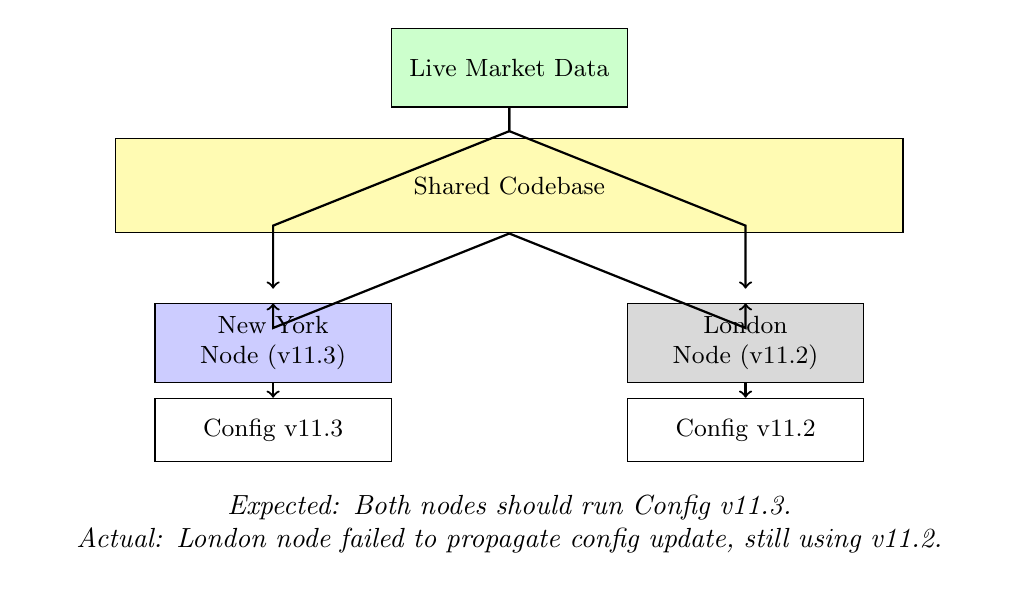
\begin{tikzpicture}[font=\small, align=center, node distance=1cm and 1cm]
  
  % Shared Codebase
  \node[draw, fill=yellow!30, minimum width=10cm, minimum height=1.2cm] (code) at (4.5, 5.5) {Shared Codebase};
  
  % Data Source
  \node[draw, fill=green!20, minimum width=3cm, minimum height=1cm] (data) at (4.5, 7) {Live Market Data};
  
  % Arrows from data to nodes
  \draw[->, thick] (data.south) -- ++(0,-0.3) -- ++(-3,-1.2) node[midway,left]{} -- ++(0,-0.8);
  \draw[->, thick] (data.south) -- ++(0,-0.3) -- ++(3,-1.2) node[midway,right]{} -- ++(0,-0.8);
  
  % New York Node
  \node[draw, fill=blue!20, minimum width=3cm, minimum height=1cm] (ny_node) at (1.5, 3.5) {New York\\Node (v11.3)};
  \node[draw, minimum width=3cm, minimum height=0.8cm] (ny_config) at (1.5, 2.4) {Config v11.3};
  \draw[->, thick] (ny_node) -- (ny_config);
  
  % London Node
  \node[draw, fill=gray!30, minimum width=3cm, minimum height=1cm] (ldn_node) at (7.5, 3.5) {London\\Node (v11.2)};
  \node[draw, minimum width=3cm, minimum height=0.8cm] (ldn_config) at (7.5, 2.4) {Config v11.2};
  \draw[->, thick] (ldn_node) -- (ldn_config);
  
  % Arrows from codebase to nodes
  \draw[->, thick] (code.south) -- ++(-3,-1.2) -- (ny_node.north);
  \draw[->, thick] (code.south) -- ++(3,-1.2) -- (ldn_node.north);
  
  % Legend/annotation
  \node[align=center, text width=12cm, font=\itshape] at (4.5, 1.2)
  {Expected: Both nodes should run Config v11.3.\\
  Actual: London node failed to propagate config update, still using v11.2.};
  
  \end{tikzpicture}
  \caption{Architecture View: Data Ingestion and Configuration Divergence Between New York and London}
\end{figure}

\medskip

\begin{TechnicalSidebar}{Configuration Files and Execution Logic}

  In modern financial systems, trading models are often split into two components:

  \medskip

  \begin{itemize}
    \item \textbf{Execution code} — the core logic that determines how trades are processed.
    \item \textbf{Configuration files} — external parameters that guide the model’s behavior: thresholds, 
    limits, feature toggles, venue preferences, and risk controls.
  \end{itemize}

  \medskip

  This separation allows developers and quants to adapt a model’s behavior without redeploying the entire 
  codebase. But it also introduces a risk: if the configuration version doesn’t match the execution context, 
  the system can behave in ways that no one intended — or approved.

  \medskip

  A famous real-world example of this happened to \textbf{Knight Capital Group} in 2012. They rolled out a new 
  trading feature across their platform — but only updated the config on 7 out of 8 machines. The eighth machine 
  retained legacy logic that had been dormant for years. 

  \medskip

  When markets opened, that single machine began firing off rogue trades at high speed. It took Knight 45 minutes 
  to identify and shut it down. However, by then, they had lost \textbf{over \$460 million}.

  \medskip

  The failure wasn’t the algorithm.

  \medskip

  It was the \textit{asymmetry between the code and its configuration}.

  \medskip

  In David’s case, a similar misalignment occurred: the London desk patched their system, but forgot to push the 
  updated configuration. As a result, they inherited a synthetic exposure that wasn’t visible in the current risk 
  profile. It had an ``invisible'' position that compliance systems couldn’t trace, and fallback logic didn’t 
  know how to limit.

\end{TechnicalSidebar}

\medskip

Behind them, the compliance pod scrambled across screens.

“Every fallback line was inherited,” Kayla continued. “TRS. OTC overlay. The routing logic defaulted to synthetic. 
That default wasn’t documented.”

David whispered to himself: “Ghost exposure…”

\medskip

\begin{TechnicalSidebar}{What is Ghost Exposure?}

  \textbf{Ghost exposure} refers to unintended, often invisible, financial risk that exists within a system — 
  but doesn’t appear in official models, dashboards, or mandate files.
  
  \medskip
  
  It can happen when:

  \medskip
  
  \begin{itemize}
    \item Configuration patches modify execution logic without being fully version-controlled.
    \item Routing defaults inherit legacy behavior from prior builds.
    \item Synthetic instruments (like TRSs or OTC wrappers) replicate risk that isn’t formally mapped.
  \end{itemize}
  
  \medskip
  
  Because these exposures aren’t visible in real-time dashboards, they bypass standard risk checks.  
  They exist in the system, but not in the \textit{assumptions} about the system.
  
  \medskip
  
  In David’s case, the fallback logic routed through synthetic channels that were technically live — but 
  undocumented in the compliance file.  
  The result: \$3 billion of “invisible” exposure, compounding losses, and no authority flagging the breach 
  until it was too late.
  
\end{TechnicalSidebar}

\medskip
  

From the wallboard, the new slippage metric blinked red.
Execution costs: +600 bps

Kayla’s voice sharpened. “London’s trying to cut the line manually—”

But she stopped.

On the wallboard, the status indicator flicked amber, then red.

David said nothing.

Because he already knew.

It was too late.

\medskip

\begin{figure}[H]
  \centering
  \begin{tikzpicture}[
      node distance=1.5cm and 1.5cm,
      auto,
      block/.style={rectangle, draw, thick, fill=blue!10, minimum width=2.8cm, minimum height=1.2cm},
      manual/.style={rectangle, draw, thick, fill=red!10, dashed, minimum width=3cm, minimum height=1.2cm},
      line/.style={draw, thick, -{Latex[length=4pt]}},
    ]

    % Nodes
    \node[block] (ingest) {Order Ingest};
    \node[block, below=of ingest] (router) {Routing Engine};
    \node[block, below left=of router, xshift=-1cm] (primary) {Primary Venue};
    \node[block, below right=of router, xshift=1cm] (synthetic) {Synthetic Route};
    \node[manual, right=2.8cm of router] (manual) {Manual Intervention};

    % Output stage
    \node[block, below=1.5cm of synthetic] (execution) {Trade Execution};

    % Edges
    \path[line] (ingest) -- (router);
    \path[line] (router) -- (primary);
    \path[line] (router) -- (synthetic);
    \path[line] (synthetic) -- (execution);
    \path[line] (primary) -- (execution);

    % Manual override line
    \draw[line, thick, red, dashed] (manual) -- (router);

    % Labels
    \node[align=center, font=\small] at ($(manual.north) + (0,0.5)$) {“Cut the line” command};
    \node[align=center, font=\small] at ($(execution.south) + (0,-0.4)$) {Final market interaction};

  \end{tikzpicture}
  \caption{System architecture showing manual intervention point in routing logic. “Cutting the line” attempts to override automated paths before execution finalizes.}
\end{figure}


\medskip

\begin{TechnicalSidebar}{What Does It Mean to ``Cut the Line Manually''?}

  In electronic trading systems, orders are routed through pre-defined execution paths — often involving layers of 
  smart order routers, synthetic strategies, and clearing intermediaries. 
  
  \medskip
  
  \textbf{Cutting the line manually} means stepping outside of automated routing to forcibly halt or reroute order flow 
  at the infrastructure level. It's like reaching for the circuit breaker when the smart thermostat isn’t responding — 
  manual override of a system that's supposed to self-govern.
  
  \medskip
  
  This can involve:

  \medskip
  
  \begin{itemize}
    \item Interrupting a FIX session or halting message flow to a broker or venue.
    \item Pulling a venue from the routing table mid-execution.
    \item Cancelling queued orders or forcibly flushing internal memory pools.
    \item Replacing dynamic routing with a hardcoded or human-validated path.
  \end{itemize}
  
  \medskip
  
  In David’s case, the model had already rerouted into synthetic space, and volumes were surging.  
  London’s attempt to cut the line manually was a last-ditch effort to regain control — but by the time they reached 
  for it, the damage was already propagating.  

  \medskip
  
  \textbf{It's too late} meant that automated systems had moved faster than the humans watching them.

\end{TechnicalSidebar}
  

\medskip

\subsection{Feedback Loop (08:39 AM)} 

The hum of the trading floor had flattened into a kind of auditory fog — no alerts, no banter, just the sound 
of ventilation and keystrokes that didn’t sound like they were helping.

David stood behind the main terminal bank, one hand pressed into his lower back, the other hovering 
over the command cluster.

“Pull updated NAV,” he said, voice low but sharp.

Julia didn’t look up. Her screen flashed, paused, then settled.

“Down thirty-two,” she said quietly. “Four billion.”

No one swore. No one moved. The number was its own gravity.

From the far end, Tom’s voice came thin through the channel.

“Portfolio liquidity’s shot. Most of the books are pinned. What’s left is slippage.”

\begin{TechnicalSidebar}{What is Slippage?}

  \textbf{Slippage} refers to the difference between the expected price of a trade and the price at which the trade 
  is actually executed.

  \medskip

  In normal market conditions, slippage might be small — just a few basis points.  
  But during high volatility or low liquidity events, slippage can spike dramatically, eroding performance and 
  compounding losses.

  \medskip

  \textbf{Why it happens:}
  \begin{itemize}
    \item Orders are too large for available market depth.
    \item The market moves while the order is being executed.
    \item Automated strategies route into thinner books or fallback venues.
  \end{itemize}

  \medskip

  In David’s case, the primary venues had dried up.  
  As the model tried to rebalance into synthetic exposure, there were fewer real buyers and sellers on the other side.  
  That meant each trade had to dig deeper into the book — crossing spreads, triggering slips, and chasing price movement.

  \medskip

  Worse still, \textit{the model didn’t stop}.  
  It kept executing based on ideal assumptions — and in doing so, made its own assumptions false.

\end{TechnicalSidebar}


Kayla leaned in from a side screen. “And synthetic margin’s ramping — hard. Every correlated leg is echoing the move.”

David frowned. “So we’re leveraged across correlation?”

\medskip

\begin{TechnicalSidebar}{Leveraging Across Correlation}

  In theory, \textbf{correlation-aware margin models} reduce capital requirements when positions appear to offset one 
  another — like being long oil and short gas. If their historical correlation is strong and inverse, the system assumes 
  reduced risk.

  \medskip

  But correlation isn’t static.  
  When the market shifts and those instruments start moving \textit{together} — not apart — the illusion of hedging collapses.

  \medskip

  \textbf{Leveraging across correlation} happens when margin algorithms treat a basket of trades as risk-neutral due to 
  historical decorrelation, but in practice, the entire basket is exposed to the same directional risk.

  \medskip

  In David’s case, the model saw multiple legs and reduced its capital requirements accordingly — giving it synthetic 
  leverage. But when the legs all began to slide the same way, the leverage \textit{amplified} losses across the entire book.

  \medskip

  What was supposed to be balanced… became synchronized.  
  And in financial systems, synchronized movement isn’t safety.  
  It’s cascade.

\end{TechnicalSidebar}

\medskip

She nodded. “Exactly. The margin model’s treating it like offsetting exposure, but it’s all in the same direction now.”

\medskip

\begin{figure}[H]
  \centering
  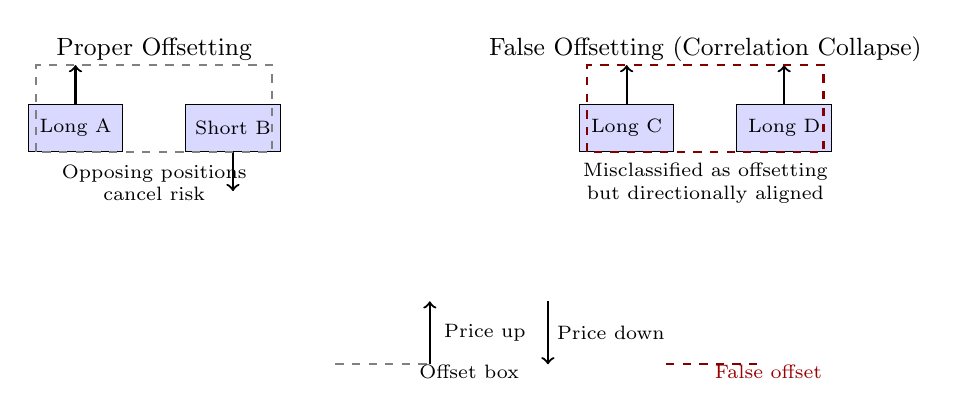
\begin{tikzpicture}[
      asset/.style={rectangle, draw=black, fill=blue!15, minimum width=1.2cm, minimum height=0.6cm, font=\scriptsize},
      arrow/.style={->, thick},
      offset/.style={dashed, thick, gray},
      netlabel/.style={font=\scriptsize, align=center}
  ]
  
  % Proper Offsetting - Left Side
  \node[font=\small, align=center] at (-3.5, 3) {Proper Offsetting};
  
  \node[asset] (longA) at (-4.5, 2) {Long A};
  \node[asset] (shortB) at (-2.5, 2) {Short B};
  
  \draw[arrow] (longA) -- ++(0,0.8);
  \draw[arrow] (shortB) -- ++(0,-0.8);
  
  \draw[offset] (-5, 1.7) rectangle (-2, 2.8);
  \node[netlabel] at (-3.5, 1.3) {Opposing positions\\ cancel risk};
  
  % False Offsetting - Right Side
  \node[font=\small, align=center] at (3.5, 3) {False Offsetting (Correlation Collapse)};
  
  \node[asset] (longC) at (2.5, 2) {Long C};
  \node[asset] (longD) at (4.5, 2) {Long D};
  
  \draw[arrow] (longC) -- ++(0,0.8);
  \draw[arrow] (longD) -- ++(0,0.8);
  
  \draw[offset, red!50!black] (2, 1.7) rectangle (5, 2.8);
  \node[netlabel] at (3.5, 1.3) {Misclassified as offsetting\\ but directionally aligned};
  
  % Legend
  \draw[arrow] (0, -1) -- ++(0,0.8);
  \node[font=\scriptsize] at (0.7, -0.6) {Price up};
  
  \draw[arrow] (1.5, -0.2) -- ++(0,-0.8);
  \node[font=\scriptsize] at (2.3, -0.6) {Price down};
  
  \draw[offset] (-1.2, -1) -- ++(1.2, 0);
  \node[font=\scriptsize] at (0.5, -1.1) {Offset box};
  
  \draw[offset, red!50!black] (3, -1) -- ++(1.2, 0);
  \node[font=\scriptsize, text=red!60!black] at (4.3, -1.1) {False offset};
  
  \end{tikzpicture}
  \caption{Proper vs False Offsetting: On the left, opposing positions reduce net exposure. On the right, assumed offsetting fails due to correlation collapse — exposing concentrated directional risk.}
\end{figure}


\medskip

\begin{TechnicalSidebar}{Offsetting Exposure}

  \textbf{Offsetting exposure} occurs when two or more positions in a portfolio counterbalance each other’s risk, allowing margin and capital models to treat the net exposure as lower than the sum of its parts.
  
  \medskip
  
  \textbf{Example:}  
  A long position in Eurodollar futures may be offset by a short in U.S. Treasury bonds, if they typically move in opposite directions under rate shifts. A margin engine may reduce the capital requirement based on their historical inverse correlation.
  
  \medskip
  
  \textbf{Why it matters:}  
  Offsetting exposure assumptions are central to portfolio margining. However, these assumptions break down when:

  \medskip

  \begin{itemize}
    \item Correlations collapse (e.g., during market stress or structural shifts),
    \item Exposures shift into the same direction due to hedging failures or correlated bets,
    \item Synthetic trades appear diverse but are functionally redundant under tail events.
  \end{itemize}
  
  \medskip
  
  \textbf{The problem:}  
  In the scenario described, the margin model is still applying an offset assumption — despite the fact that all legs of the trade are now aligned directionally. This creates a dangerous illusion of balance where none exists.

  \medskip
  
  \textbf{Result:}  
  Underpricing of risk, underestimation of drawdown, and delayed escalation — until the margin engine snaps.
  
\end{TechnicalSidebar}

\medskip

Julia’s fingers danced over her console. “Model’s rebalancing. It’s—” she paused. “It’s accelerating the drawdown.”

David closed his eyes for half a second. The kind of blink that tries to erase the moment but finds it waiting.


“Pull the rebalance queue,” he said.

“It’s already executing,” Julia said. “TRS, OTC, and overlay legs. It thinks it's stabilizing.”

“But it’s not,” David said flatly.

Kayla tapped her screen again. “It’s fighting the fire with gasoline.”

The floor was silent again.

In the corner, a junior whispered: “How far does it go?”

No one answered.

\medskip

\begin{tcolorbox}[title=Silent Failure Modes, colback=gray!5, colframe=black]
Silent failures occur when fallback systems activate without signaling — no exception raised, no error thrown.\\
What looks like successful execution may, in fact, be catastrophic redirection.\\
In distributed systems, this is often the most dangerous kind of failure — because it looks like success until it’s too late.
\end{tcolorbox}

\medskip

\subsection{Too Late To Matter (08:57 AM)} 

The glass on the east side of the trading floor had gone gold — not with warmth, but with the sharp, 
sterile glow of a mid-morning sun that hadn’t been invited.

David was standing. Again. Still.

The floor was silent except for the low mechanical purr of the HVAC and the soft ticking of trades 
that no longer meant anything.

Julia's voice came without emotion. “Kill switch just triggered.”

David didn’t respond immediately. His eyes stayed fixed on the execution wall, where synthetic 
volume had finally collapsed — not from relief, but from absence.

He inhaled once, then: “What’s the NAV?”

Kayla glanced sideways. “Down forty.”

He blinked. “Five billion.”

“Yeah,” she said. “Cross-routing delay bought the drawdown an extra five minutes.”

David’s hand hovered over the desk console, fingers slightly curled — not ready to type, not willing to leave.

“Latency?”

“Confirmed,” said Julia. “Jurisdictional lag. London’s desk tried to reconcile exposure before halt propagation.”

David exhaled through his nose. “So the switch was waiting on a bookkeeping round-trip.”

\medskip

\begin{TechnicalSidebar}{Bookkeeping Round-Trip}

  In high-speed trading and risk systems, a \textbf{bookkeeping round-trip} refers to the complete cycle in which a 
  trade or exposure adjustment is:

  \medskip
  
  \begin{enumerate}
    \item \textbf{Logged} locally in a regional system (e.g., London),
    \item \textbf{Transmitted} to a central ledger or compliance database (often in a different legal jurisdiction),
    \item \textbf{Validated}, reconciled, or transformed by risk or reporting modules,
    \item And finally, \textbf{Returned} with confirmation to the originating node.
  \end{enumerate}

  \medskip
  
  This delay — sometimes only a few seconds under normal conditions — can stretch under heavy system load or fragmented 
  architecture.

  \medskip
  
  \textbf{Why it matters:} During a crisis, kill switches or exposure thresholds may be programmed to wait for this 
  round-trip completion before executing a halt or alert. In this case, that design introduced a fatal lag: while London 
  waited for confirmation, the system continued to hemorrhage value.

  \medskip
  
  \textbf{Analogy:} It’s like trying to slam on the brakes — but waiting for your co-driver to finish checking the 
  rearview mirror first.

\end{TechnicalSidebar}

\medskip

Tom’s voice crackled through the channel from Compliance. “Kill code was clean. But the signal didn’t clear.  
Too many routes still open. I see synthetic, OTC, TRS. System doesn't recognize it as final.”

David closed his eyes.

Five billion gone. Not in a panic. In logic. In routing delays and trust in fallbacks that never came.

David whispers, “Too late to matter.”

No one corrected him.

David stares at the terminal.

He had scoped the risk.  
But not the fallback.
Not the latency.
Not the new routing path.
Not the architecture his name now sat atop.

Regulators later called it a \textbf{configuration control failure}.

Because the memo said ring-fenced.

But the implementation crossed jurisdictions.

And the safeguards weren’t centralized.

\textbf{And David had initialed the memo.}

\medskip

\begin{figure}[H]
  \centering
  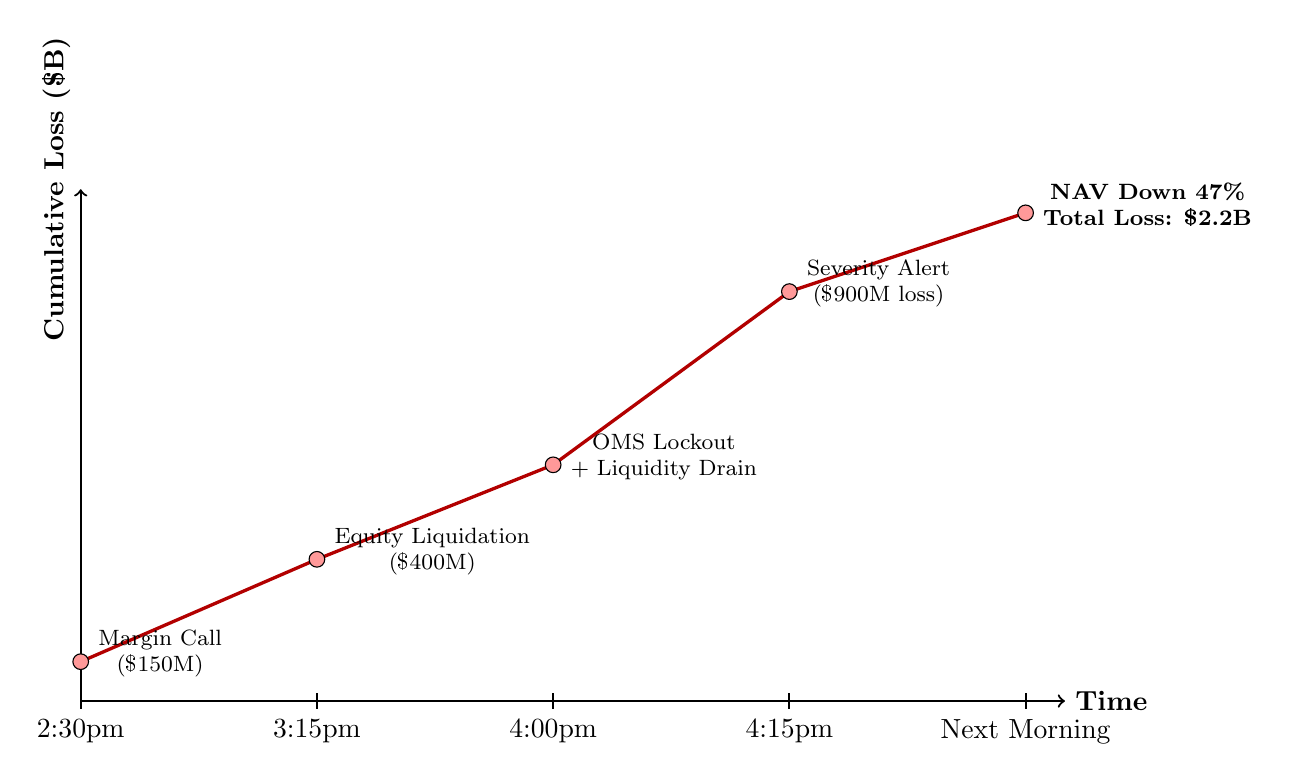
\begin{tikzpicture}[
    scale=1,
    axis/.style={thick, ->},
    event/.style={font=\footnotesize, align=center},
    loss/.style={circle, fill=red!40, draw=black, minimum size=4pt, inner sep=2pt}
  ]
  
  % Axes
  \draw[axis] (0,0) -- (12.5,0) node[right] {\textbf{Time}};
  \draw[axis] (0,0) -- (0,6.5) node[above, rotate=90] {\textbf{Cumulative Loss (\$B)}};
  
  % Time markers
  \foreach \x/\label in {
    0/2:30pm,
    3/3:15pm,
    6/4:00pm,
    9/4:15pm,
    12/Next Morning
  } {
    \draw[thick] (\x,0.1) -- (\x,-0.1) node[below] {\label};
  }
  
  % Loss line
  \draw[very thick, red!70!black]
    (0,0.5) 
    -- (3,1.8) 
    -- (6,3.0) 
    -- (9,5.2)
    -- (12,6.2);
  
  % Dots on line
  \node[loss] at (0,0.5) {};
  \node[loss] at (3,1.8) {};
  \node[loss] at (6,3.0) {};
  \node[loss] at (9,5.2) {};
  \node[loss] at (12,6.2) {};
  
  % Annotations
  \node[event, anchor=west] at (0.1,0.6) {Margin Call\\(\$150M)};
  \node[event, anchor=west] at (3.1,1.9) {Equity Liquidation\\(\$400M)};
  \node[event, anchor=west] at (6.1,3.1) {OMS Lockout\\+ Liquidity Drain};
  \node[event, anchor=west] at (9.1,5.3) {Severity Alert\\(\$900M loss)};
  \node[event, anchor=west] at (12.1,6.3) {\textbf{NAV Down 47\%}\\\textbf{Total Loss: \$2.2B}};
  
  \end{tikzpicture}
  \caption{Escalating Cumulative Loss: Arcadia's collapse unfolded in phases, each compounding the damage.}
\end{figure}

\medskip





